\chapter{LHC y detector ATLAS}
% \addcontentsline{toc}{chapter}{LHC y detector ATLAS}



\chaptermark{LHC y detector ATLAS}




El Gran Colisionador de Hadrones (\textit{\textbf{L}arge \textbf{H}adron \textbf{C}ollider} (LHC)) \cite{Evans:1129806} es el acelerador de hadrones de la Organización Europea para la Investigación Nuclear (CERN, por su antigua sigla en francés), ubicado en la frontera entre Francia y Suiza. El mismo consiste en un anillo de \magn{27}{km} de circunferencia construido en el mismo túnel en el que funcionaba el acelerador $e^{+}e^{-}$ LEP (entre 1989 y 2000) \cite{LEPbook}, a una profundidad variable entre \magn{50}{m} y \magn{174}{m} de la superficie.

El LHC está diseñado para colisionar protones a un máximo de energía de centro de masa\footnote{Definida como la raíz cuadrada de la variable de Mandelstan, $\sqrt{s}=|p_1+p_2|$, donde $p_1$ y $p_2$ representan los cuadrimomentos de las partículas incidentes.} de \com{14}{TeV}. Para ello el CERN posee un complejo de aceleradores que en sucesivas etapas incrementan la energía de los protones, para luego inyectarlos en el LHC y hacerlos colisionar en cuatro puntos distintos donde se encuentran los detectores más importantes: ATLAS \cite{PERF-2007-01}, CMS \cite{CMS}, LHCb \cite{LHCb} y ALICE \cite{ALICE}.

La producción de protones comienza extrayendo los electrones de un contenedor con gas de hidrógeno mediante campos magnéticos. Luego los protones pasan por un complejo de aceleradores que en el pasado funcionaban como experimentos y que actualmente se utilizan para incrementan la energía de los protones en sucesivas etapas, como muestra la Figura \ref{fig:LHC_complex}. Inicialmente los protones son inyectados al acelerador lineal LINAC 2, que mediante cavidades de radiofrecuencia, acelera a los protones a una energía de \magn{50}{MeV}. Desde aquí son dirigidos al \textit{Proton Synchrotron Booster} que consiste en cuatro anillos superpuestos con un radio de \magn{25}{m} que aceleran los protones hasta una energía de \magn{1.4}{GeV}. Este último inyecta los protones en el \textit{Proton Synchroton}, cuya circunferencia de \magn{628}{m} e inyecta protones de hasta \magn{26}{GeV} en el \textit{Super Proton Synchroton}, y este a su vez tiene una circunferencia de \magn{7}{km} e inyecta protones de hasta \magn{450}{GeV} en ambos anillos del LHC. 

\begin{figure}
  \centering
  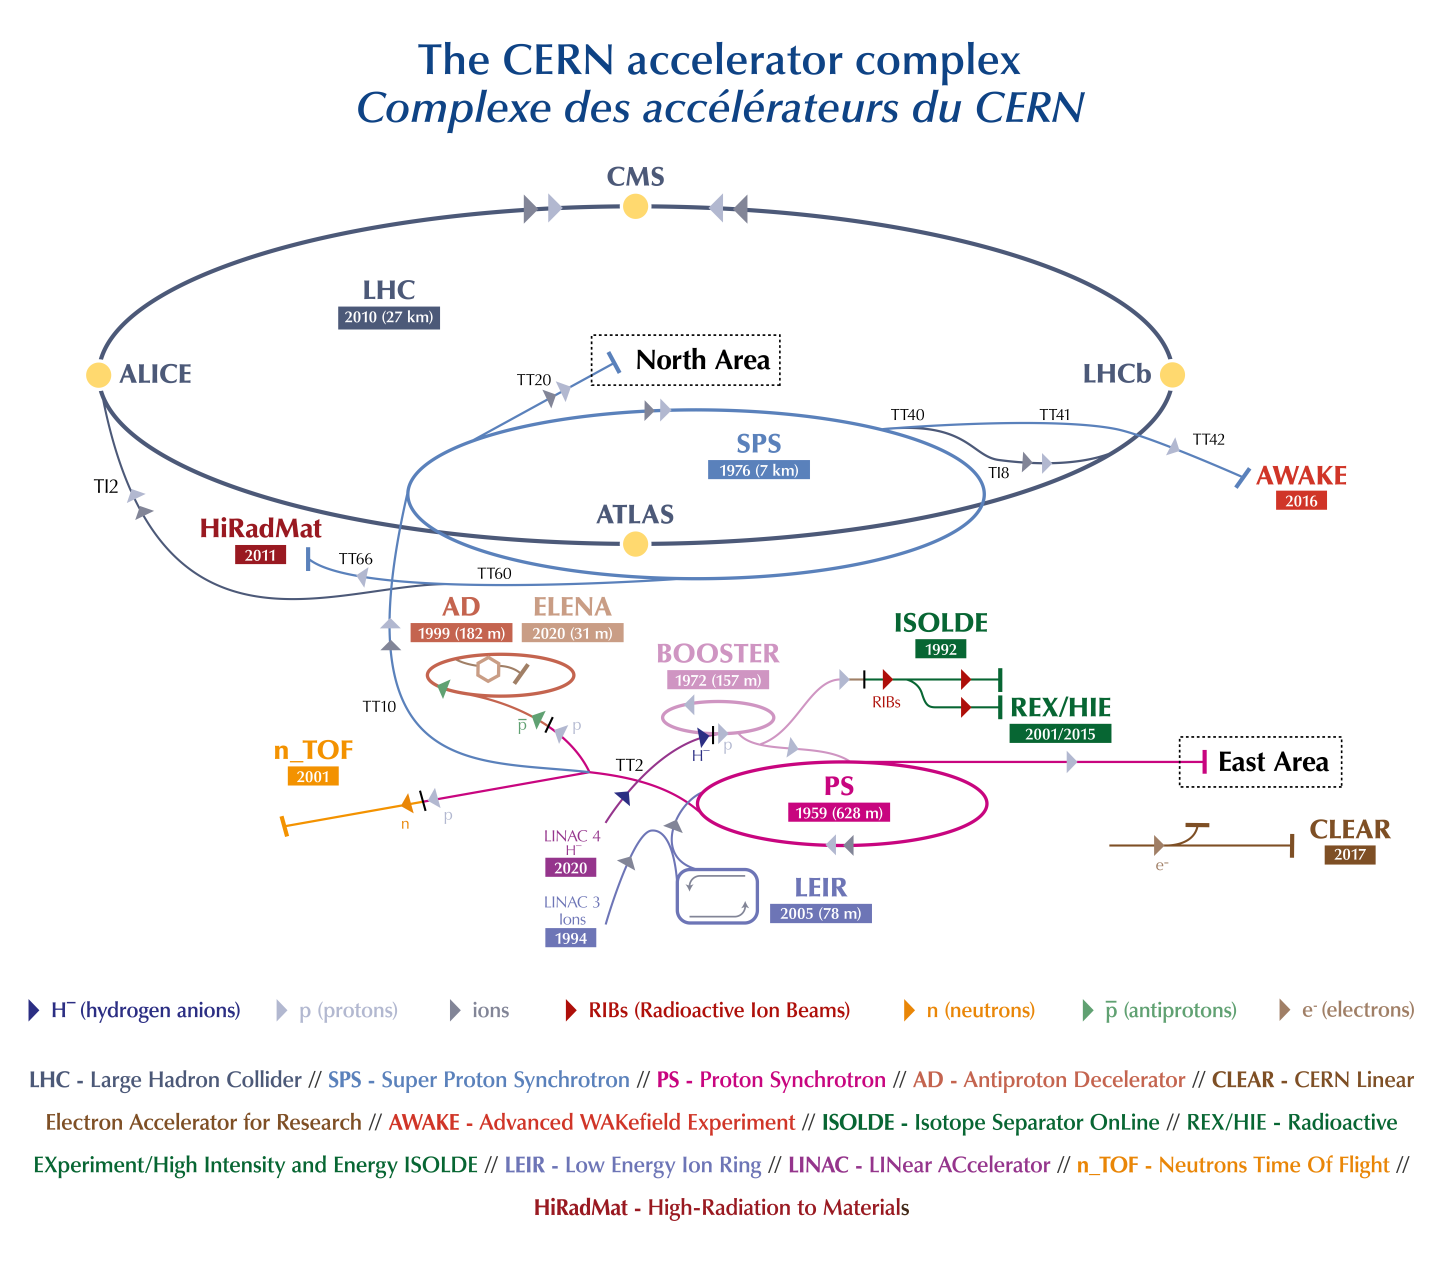
\includegraphics[width=0.65\textwidth]{images/lhc/LHC_complex.png}
  \caption{Complejo de aceleradores del LHC \cite{Lopienska:2800984}.}
  \label{fig:LHC_complex}
  % https://cds.cern.ch/record/2684277?ln=es
  % https://cds.cern.ch/images/CERN-GRAPHICS-2022-001-1
\end{figure}

El último de los aceleradores es el LHC, donde los protones circulan en direcciones opuestas por cavidades de ultra alto vacío a una presión de \magn{$10^{-10}$}{torr}. El mismo cuenta con $1232$ dipolos magnéticos superconductores de \magn{15}{m} de largo enfriados a \magn{1.9}{K} mediante helio superfluído, que generan un campo magnético de $8.4$ T y permiten mantener en su órbita circular a los protones. Los dipolos están equipados con sextupolos, octupolos y decapolos, que permiten corregir las pequeñas imperfecciones del campo magnético en las extremidades de los dipolos. Para aumentar la probabilidad de colisión, existe un sistema de focalización de los haces en las proximidades de los detectores, que estrecha el camino que recorren los protones. El mismo consiste de $392$ cuadrupolos magnéticos que generan campos magnéticos de \magn{6.8}{T}.

Los protones son acelerados mediante cavidades de radiofrecuencia que generan una diferencia de potencial longitudinal a una frecuencia específica. En esa frecuencia los protones sincronizados con la energía deseada no van sufrir aceleración alguna, mientras que aquellos desincronizados van a ser acelerados o desacelerados hasta obtener la energía deseada. De esta forma el haz de protones se divide en paquetes discretos denominados \textit{bunches}, cada uno conteniendo del orden de 10$^{11}$ protones. El número de paquetes totales posibles en un haz con un espaciado de \magn{25}{ns} es de 3564 \footnote{Se obtiene al dividir la frecuencia de las cavidades, \magn{400}{MHz}, por la frecuencia de revolución, \magn{11}{kHz}, y considerando que sólo 1 de cada 10 paquetes es llenado para lograr el espaciado deseado}. Considerando los tiempos que se necesitan para en la inyección y descarte del haz, junto con los tiempos que necesita cada detector para procesar la información, no todos los paquetes son llenados, sino que se dejan `espacios' definidos por diferentes esquemas, dejando así el número efectivo de paquetes llenos a 2808.

Los aceleradores pueden ser caracterizados no solo por su energía de centro de masa sino también por su luminosidad instantánea ($\mathcal{L}$), que mide el número de colisiones por unidad de área que ocurren en un período de tiempo y se define como: 

\begin{equation}
\mathcal{L}= \frac{1}{\sigma}\frac{dR}{dt} = f_{\text{rev}}n_{b}\frac{N_{1}N_{2}}{A}
\end{equation}

\noindent
donde $\sigma$ es la sección eficaz de la colisión y $R$ el número de colisiones. La expresión se puede escribir para el caso de un acelerador circular como el LHC, donde $f_{\text{rev}}$ es la frecuencia de revolución ($\sim$\magn{11}{kHz}), $n_{b}$ es el número de paquetes por haz, $N_{i}$ es el número de partículas en cada paquete y $A$ es la sección efectiva del haz, que puede expresarse en término de los parámetros del acelerador como:

\begin{equation}
A=\frac{4 \pi \epsilon_{n}\beta^{*}}{\gamma F}
\end{equation} 

\noindent
donde $\epsilon_{n}$ es la emitancia transversal normalizada (la dispersión transversal media de las partículas del  haz en el espacio de coordenadas e impulsos), $\beta^{*}$ es la función de amplitud en el punto de interacción (relacionada al poder de focalización de los cuadrupolos), $\gamma$ es el factor relativista de Lorentz y $F$ es un factor de reducción geométrico, debido al ángulo de cruce de los haces en el punto de interacción.

El número total de eventos esperados para un dado proceso con una sección eficaz $\sigma$, se obtiene como:

\begin{equation}
N=\sigma \int \mathcal{L} dt = \sigma \mathcal{L}_{\text{int}}
\label{eq:lumi_xs}
\end{equation}	

\noindent
donde al factor integral se lo conoce como luminosidad integrada.

El LHC comenzó a funcionar en 2009 en lo que se denominó \textit{Run 1}. Durante el 2011 se realizaron colisiones a una energía de de centro de masa de \magn{7}{TeV}, y durante el 2012 a \magn{8}{TeV}, logrando finalmente recolectar una luminosidad total integrada de \magn{28.2}{\ifb} \cite{DAPR-2011-01,DAPR-2013-01}, que era apta para análisis físicos \footnote{El termino `apto para física' hace referencia a los datos que pasaron una selección de calidad mínima para ser empleados en análisis físicos, y naturalmente son menores a los detectados por ATLAS y más aún a los proveídos por el LHC.}. En el 2013 finaliza la toma de datos y comienza el \textit{Long shutdown 1}, período que se utilizó para realizar distintas actualizaciones tanto al LHC como a los detectores, y preparándose así para la siguiente toma de datos. En el 2015 comenzó el \textit{Run 2} que operaba a una energía de de centro de masa de \magn{13}{TeV} y proveyendo una luminosidad total integrada de \magn{139}{\ifb} \cite{lumi_13tev}, para luego finalizar en el 2018 y dar lugar al \textit{Long shutdown 2}. Este último estaba previsto con una duración de dos años, pero dada la situación epidemiológica de COVID-19 el mismo se terminó extendiendo hasta 2022.
Los planes a futuro del LHC preveen un \textit{Run 3} a \magn{14}{TeV} de tres años de duración aproximada, y luego ingresar en un nuevo período de inactividad para realizar las mejoras necesarias para el \textit{High Luminosity LHC} (HL-LHC). En la Figura \ref{fig:lhc_periods} se puede observar un diagrama de los períodos del LHC desde el Run 1 hasta el HL-LHC. La Figura \ref{fig:run2_lumi} muestra la luminosidad total integrada acumulada durante los días correspondientes al Run 2.

\begin{figure}
  \centering
  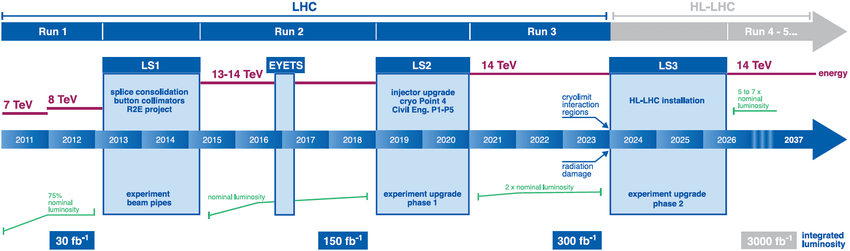
\includegraphics[width=0.9\textwidth]{images/lhc/lhc_periods.png}
  \caption{Períodos del LHC desde el Run 1 hasta el futuro HL-LHC. Se detalla en cada período de toma de datos, la energía de centro de masa y la luminosidad total proveída por el LHC \cite{lhc_periods}.}
  \label{fig:lhc_periods}
\end{figure}

\begin{figure}
  \centering
  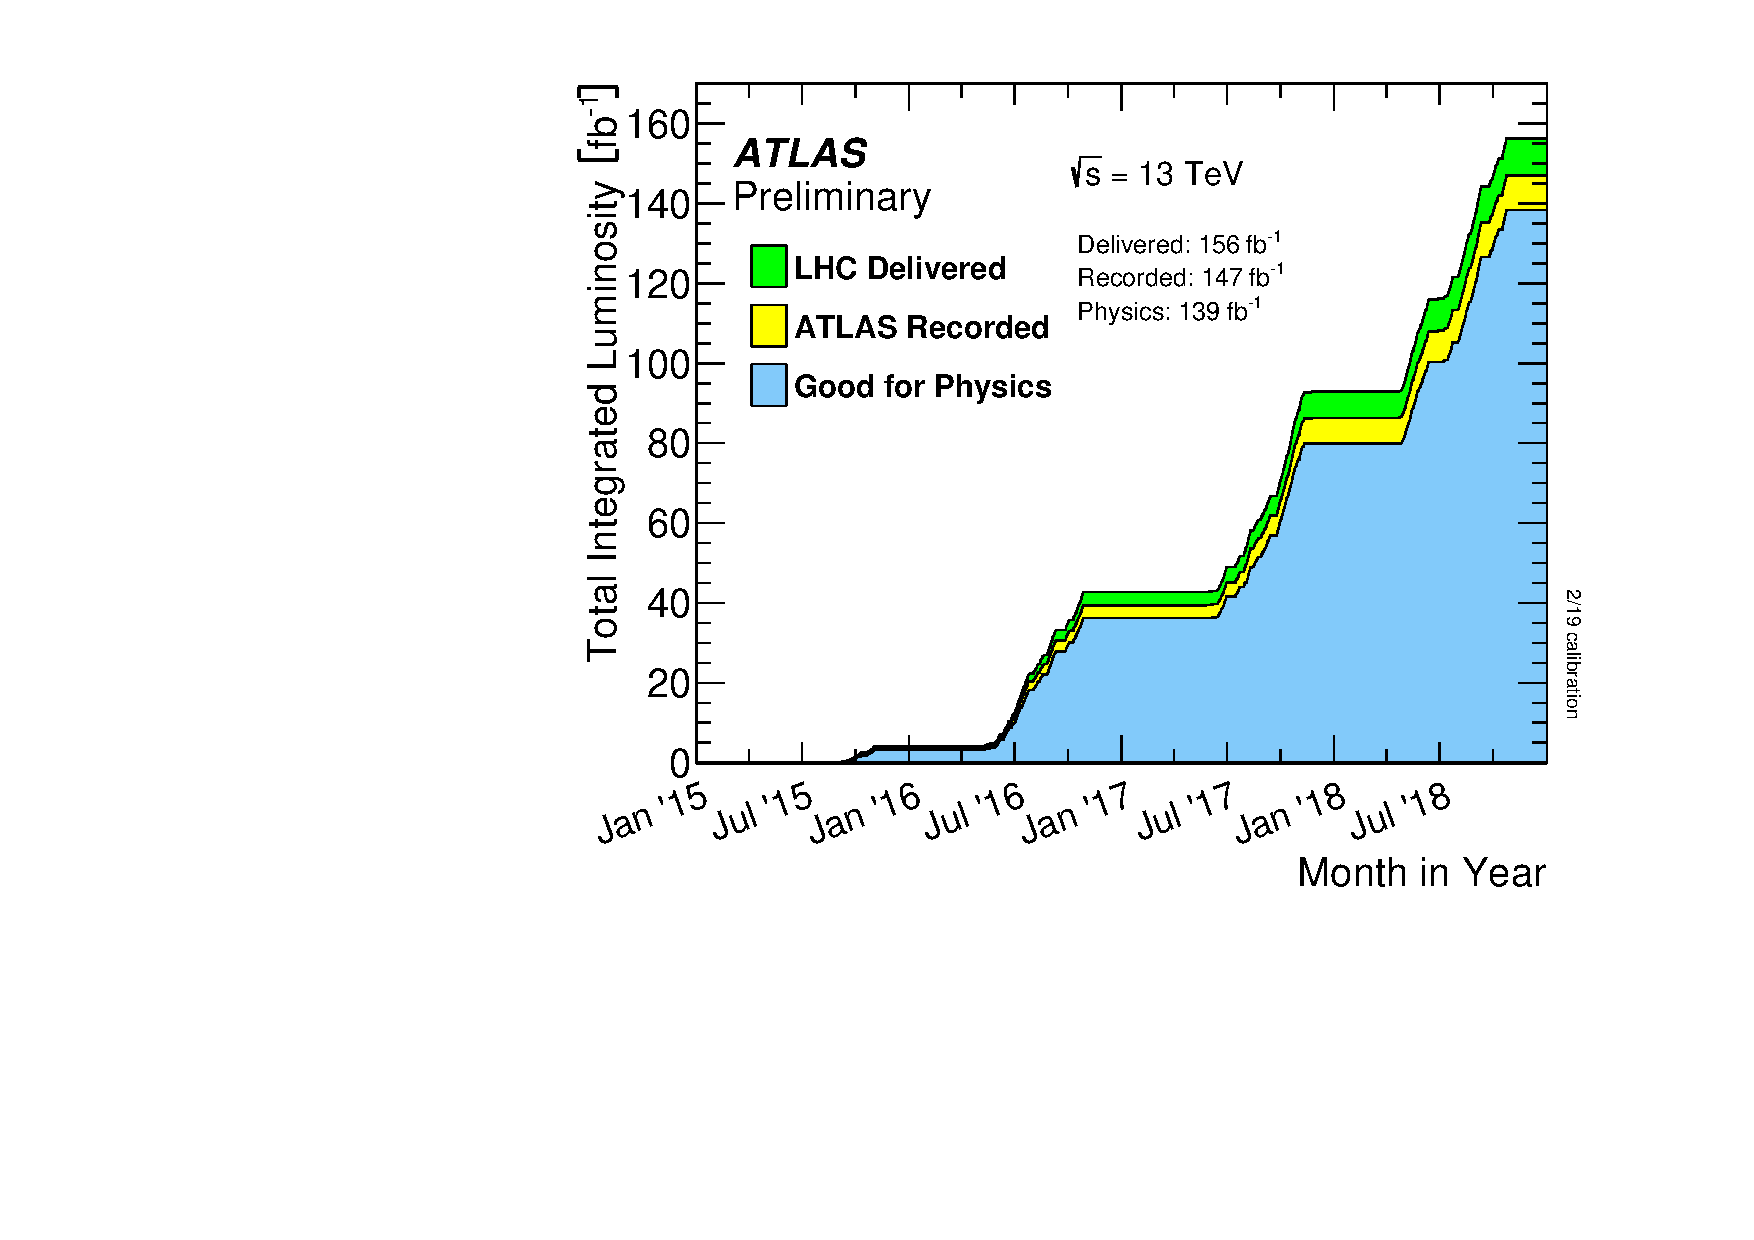
\includegraphics[width=0.8\textwidth]{images/lhc/intlumivstimeRun2DQall.pdf}
  \caption{Luminosidad total integrada acumulada durante los días del Run 2 \cite{lumi_plot}. Se muestra la luminosidad proveída por el LHC (verde), la detectada por ATLAS (amarillo) y la apta para análisis físicos (celeste).}
  \label{fig:run2_lumi}
\end{figure}

Las nuevas condiciones del Run 2 significaron un desafío para la toma de datos, en particular el incremento de \textit{pile-up}, que se define como el número promedio de interacciones por cruce de paquetes ($\langle \mu \rangle$). Cuando se cruzan dos paquetes de protones, varios protones de los mismos pueden interactuar, generando múltiples vértices primarios (\textit{in-time} pile-up). Esto dificulta la reconstrucción de los objetos del evento, debido a que la trayectoria de los mismos debe estar correctamente asociada a su correcto vértice. Inclusive puede ocurrir la superposición de señales provenientes del paquete anterior o posterior, lo que implica una nueva dificultad. Estos efectos están contemplados en los dinstintos algoritmos de recotrsucción de obetos que se describen en el Capítulo \ref{cap:objects}. En la Figura \ref{fig:pileup} se puede observar el número promedio de interacciones por cruce de paquetes durante el Run 2. Allí se observa que en promedio se tuvieron 30 interacciones por cruce, y hasta un máximo de 70. 

\begin{figure}
  \centering
  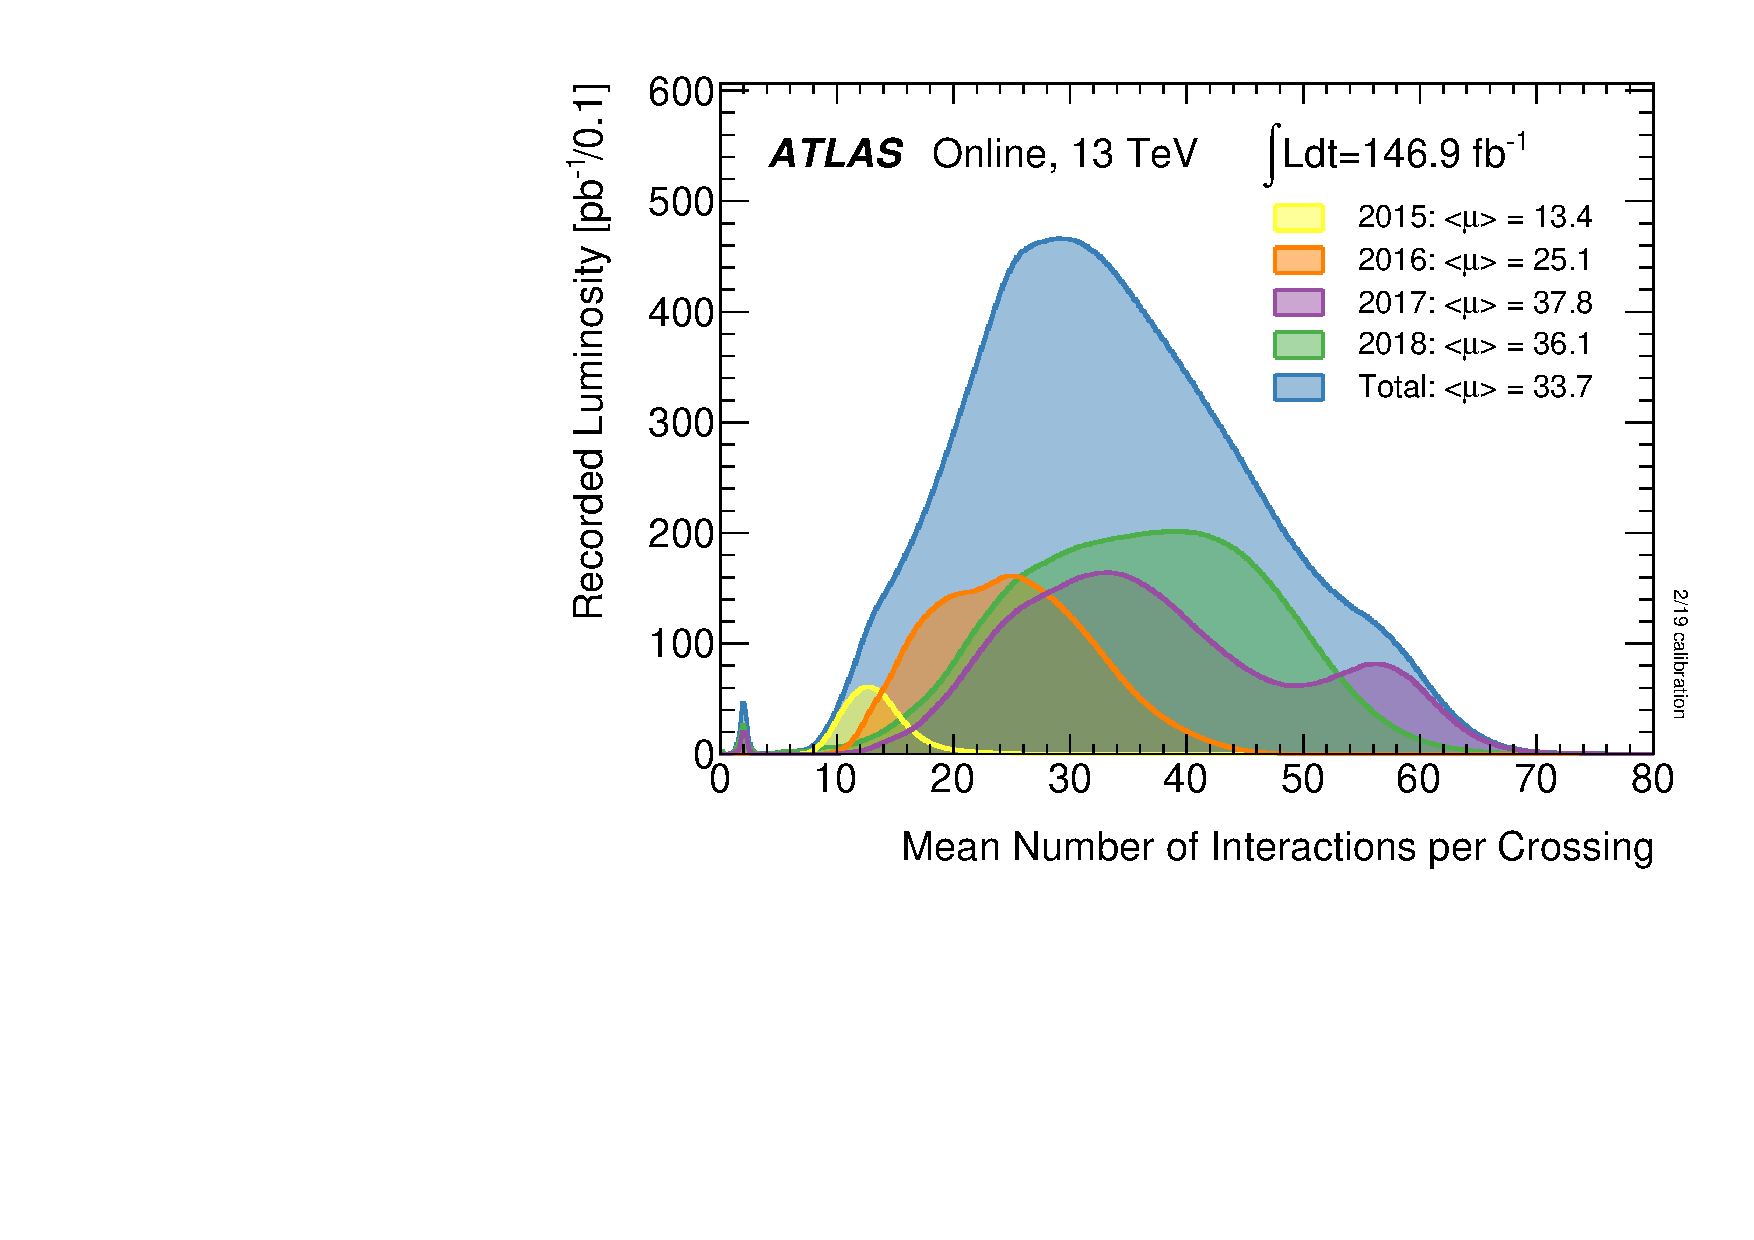
\includegraphics[width=0.8\textwidth]{images/lhc/mu_2015_2018.pdf}
  \caption{Interacciones por cruce de paquetes promedio durante el Run 2 \cite{lumi_plot}.}
  \label{fig:pileup}
\end{figure}

\section{El detector ATLAS}


ATLAS (\textit{\textbf{A} \textbf{T}oroidal \textbf{L}HC \textbf{A}pparatu\textbf{S}})  \cite{PERF-2007-01} es uno de los experimentos multipropósito del LHC, diseñado para estudiar las colisiones protón-protón a altas energías provistas por el LHC. El mismo tiene una simetría aproximadamente cilíndrica y está compuesto de distintos subdetectores, que cumplen diversas funciones en la identificación de las partículas producidas durante las colisiones. 

En la zona más próxima al haz se encuentra detector interno de trazas (ID) cuyo objetivo principal es reconstruir la trayectoria de las partículas cargadas. Está compuesto del \textit{Insertable B-Layer} (IBL), un detector de píxeles, un detector de bandas de silicio (SCT) y un detector de radiación de transición (TRT). A su vez, envolviendo al ID, se encuentra un solenoide superconductor que genera un campo magnético de \magn{2}{T}, el cual curva la trayectoria de las partículas cargadas permitiendo así medir su impulso. A continuación se ubica el sistema de calorímetros compuesto por el calorímetro electromagnético (ECAL) que mide principalmente la energía depositada por fotones y electrones, y el calorímetro hadrónico (HCAL) para medir la energía de los jets y hadrones. En la parte más externa, se encuentra el espectrómetro de muones (MS) diseñado para detectar la producción de muones y además medir su momento. Este último es el que le da a ATLAS su tamaño característico de \magn{45}{m} de largo y \magn{25}{m} de alto. Intercalado con el MS se encuentra un sistema de imanes toroidales, que generan un campo magnético de \magn{4}{T} para curvar la trayectoria de los muones hacia el final del detector.

El detector ATLAS se divide geométricamente en dos regiones, la parte central denominada \textit{barrel} y la región extrema denominada \textit{endcap}. En la región barrel los detectores se ubican en forma de cilindros concéntricos alrededor del eje del haz, mientras en la región endcap se disponen como discos perpendiculares a la dirección del haz. La Figura \ref{fig:atlas_1} detalla todas las componentes que integran al detector ATLAS y son descriptas en detalle a en las siguientes secciones.

\begin{figure}
\centering
  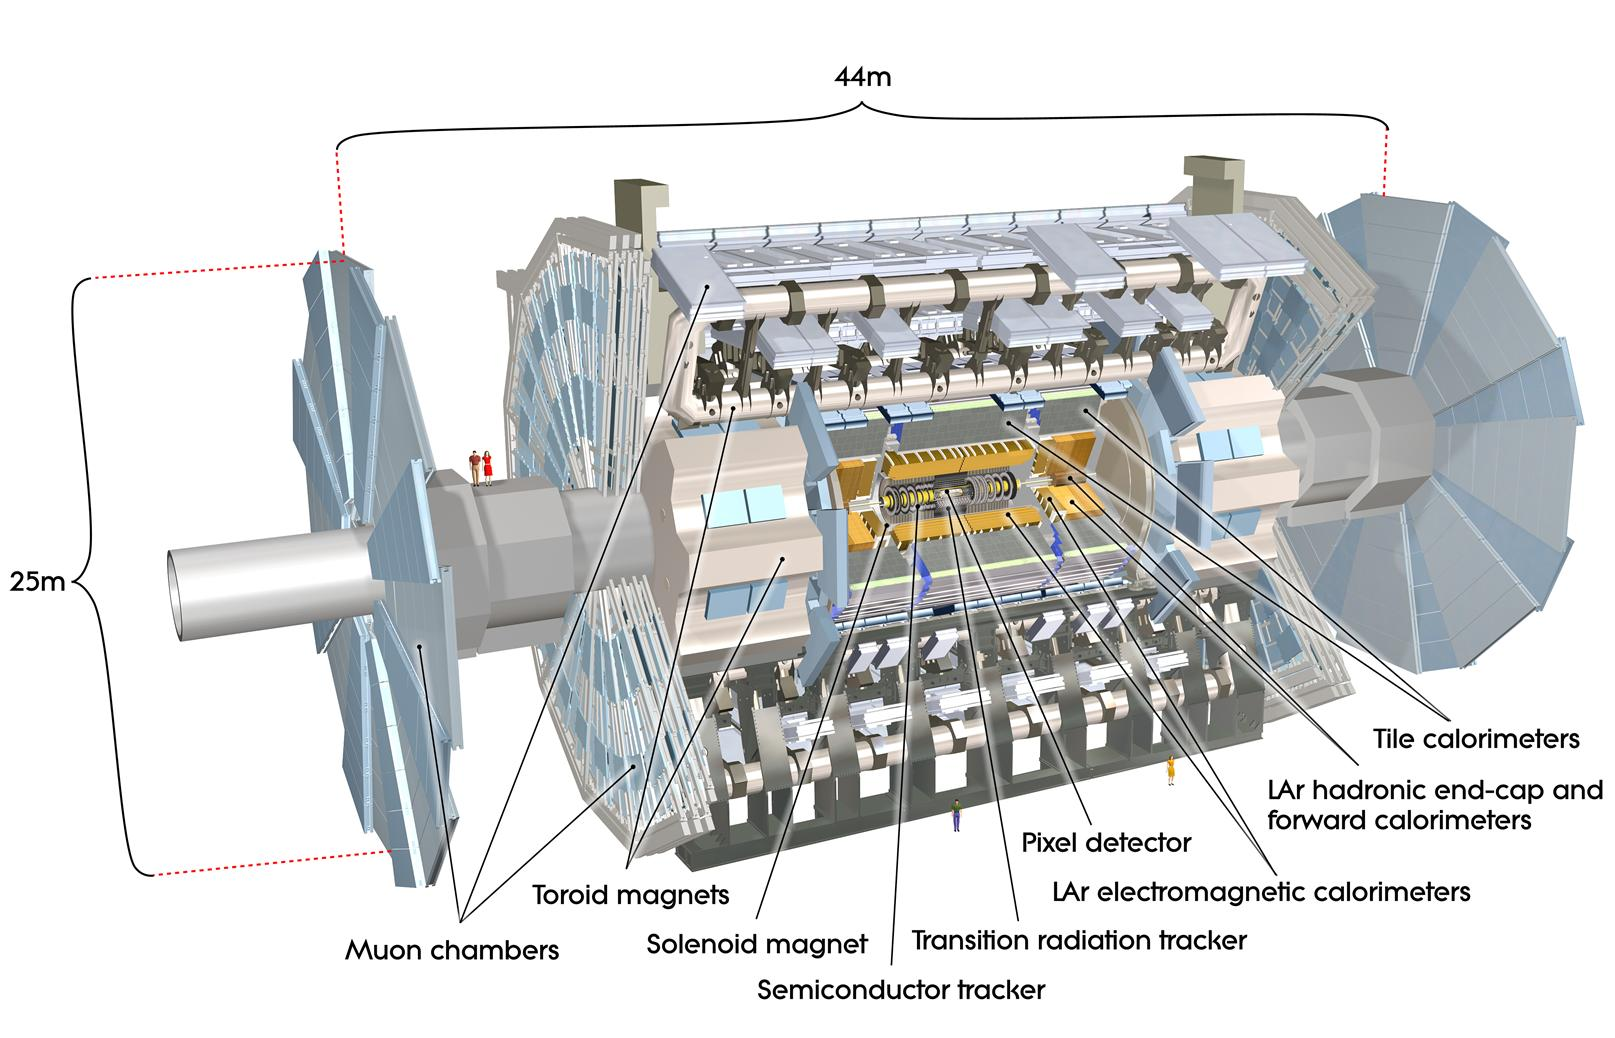
\includegraphics[width=0.9\textwidth]{images/lhc/atlas_1.jpg}
  \caption{Esquema del detector ATLAS, indicando cada uno de los subdetectores que lo componen \cite{Pequenao:1095924}.}
  \label{fig:atlas_1}
\end{figure}

\section{Sistema de coordenadas}

El sistema de coordenadas de ATLAS corresponde a un sistema cartesiano, cuyo origen coincide con el punto de interacción nominal ubicado en el centro del detector. El eje $z$ está orientado con hacia la dirección del haz, el eje $x$ se define desde el punto de interacción hacia el centro del anillo del LHC, y el eje $y$ se define apuntando hacia la superficie terrestre. Es conveniente además definir un sistema de coordenadas cilíndricas donde el radio $R$ representa la distancia perpendicular al haz, el ángulo azimutal $\phi$ es medido alrededor del eje del haz, y $\theta$ es el ángulo con respecto al eje $z$. La Figura \ref{fig:atlas_coordinates} muestra un diagrama del sistema de coordenadas de ATLAS.

\begin{figure}
\centering
  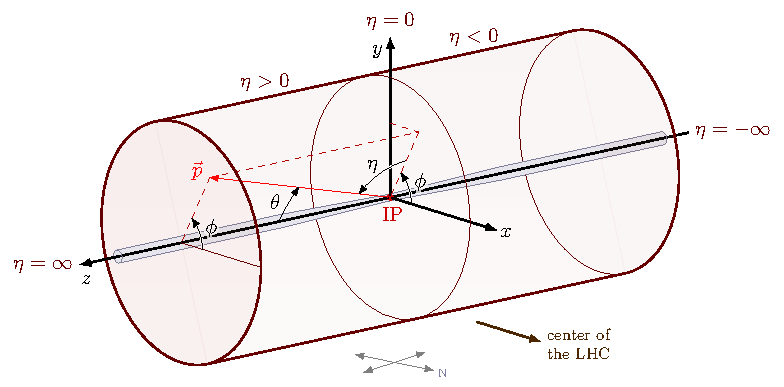
\includegraphics[width=0.8\textwidth]{images/lhc/atlas_coordinates2.pdf}
  \caption{Esquema del detector ATLAS, indicando cada uno de los subdetectores que lo componen \cite{atlas_coordinates}.}
  % https://tikz.net/axis3d_cms/
  \label{fig:atlas_coordinates}
\end{figure}


Una variable utilizada en física experimental de altas energías es la rapidez:

\begin{equation}
y=\frac{1}{2}\ln\left( \frac{E+p_{z}}{E-p_{z}}\right)
\end{equation}

\noindent
donde $E$ es la energía total de la partícula y $p_{z}$ es la componente en la dirección del haz de su impulso\footnote{Esta definición es un caso particular de la rapidez utilizada en relatividad especial, cuando se realiza una transformación en la dirección del haz del sistema de laboratorio a un sistema donde la partícula solo se mueve perpendicular al haz.}. En el límite de altas energías, en donde la masa de la partícula es despreciable frente a su momento, es posible aproximarla a la llamada pseudorapidez $\eta$:

\begin{equation}
\eta =-\ln \tan\left( \frac{\theta}{2} \right)
\end{equation}

\noindent
estando completamente relacionada con el ángulo $\theta$. La razón detrás de esta transformación de coordenadas se debe a que
 % \tosolve{consultar}
 % Lo vi en la tesis de fran y en wikipedia pero dice `loosely speaking' y no entiendo bien a qué se refiere.
 % Basicamente la cantidad de particulas que se produce esta mas concetrada en la region forward, al hacer esta variable dependiente de pt como que se distribuye de forma uniforme...
 la multiplicidad de partículas producidas es aproximadamente constante como función de $\eta$, y que 
 la diferencia de pseudorapidez entre dos partículas es invariante frente a transformaciones de Lorentz a lo largo de la dirección del haz. 

% dR, ???
% parrafor que viene similar a tesis de lic, que es basicamente la tesis de fran: ya modificado!

Como se mencionó anteriormente, al considerar colisiones hadrónicas de altas energías se hace uso del modelo de partones. Los partones acarrean una fracción del momento inicial de los hadrones, que a priori es desconocida. Si bien es posible medir una parte de ese momento, principalmente de los partones interactuantes que conforman la interacción fuerte, hay una fracción que escapa la detección. Esto imposibilita la reconstrucción del movimiento longitudinal del centro de masa en la interacción, y hacer uso de leyes de conservación sobre la cinemática total del evento. En cambio, teniendo en cuenta que el momento total de los partones en la dirección transversa al haz es nulo, el impulso total transverso se debe conservar durante la colisión. Por tal motivo, es común utilizar solo las componentes transversales en la descripción de la cinemática del evento, definidas en términos de la pseudorapidez, como por ejemplo el momento transverso:

\begin{equation}
p_{T}=p\sin\theta=\frac{p}{\cosh{\eta}}
\end{equation}

\noindent
donde $p$ es el momento de la partícula. De esta forma es posible describir la cinemática de cada partícula en términos de ($\pt$, $\eta$, $\phi$)

\section{Sistema de imanes}

El detector ATLAS posee un poderoso sistema de imanes \cite{magnet} utilizado para curvar la trayectoria de las partículas cargadas, pudiendo así medir tanto su impulso de forma precisa como también su carga. El mismo consta de dos tipos de imanes superconductores, uno en forma solenoidal y otros tres forma toroidal, enfriados a una temperatura de \magn{4.5}{K} para poder producir los fuertes campos magnéticos.

El solenoide rodea al detector interno, y tiene un tamaño de \magn{5.6}{m} de largo y \magn{2.56}{m} de diámetro, 
y con un espesor de apenas \magn{4.5}{cm}. El mismo produce un campo magnético de $\sim$\magn{2}{T} en la dirección del haz, por lo que las partículas cargadas son curvadas en la dirección de $\phi$. Para minimizar la interacción de las partículas que lo atraviesan y ahorrar la mayor cantidad de material posible, el solenoide comparte la cámara de vacío del calorímetro de argón líquido (LAr) descripto en las siguientes secciones.

Los toroides de ATLAS se componen de ocho bobinas, que generan campos de hasta $\sim$\magn{4}{T} en la dirección $\phi$, por lo que las partículas que lo atraviesan (prácticamente solo muones) son curvadas en la dirección $\eta$. El más grande de ellos mide \magn{25.3}{m} de largo y \magn{20.1}{m} de diámetro, y se ubica en la parte más externa del detector barrel intercalado con el Espectrómetro de Muones descripto en las siguientes secciones. Los otros dos restantes se encuentran en la región endcap, por fuera de los calorímetros, y miden \magn{5}{m} de largo y \magn{10.7}{m} de diámetro. La Figura \ref{fig:magnet_1} muestra el esquema de imanes del detector ATLAS.

\begin{figure}
\centering
  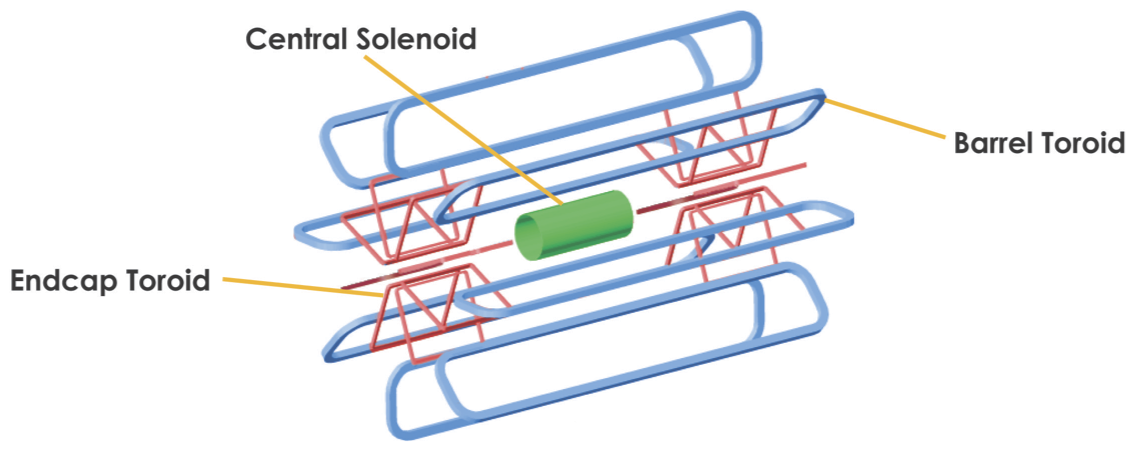
\includegraphics[width=0.8\textwidth]{images/lhc/magnet_1.png}
  \caption{Sistema de imanes del detector ATLAS \cite{magnet_system}.}
  \label{fig:magnet_1}
\end{figure}


\section{Los subdetectores de ATLAS}

\subsection{Detector interno}

El detector interno es el más próximo al haz y su función principal es la reconstrucción de las trazas de las partículas cargadas, que a su vez sirve para medir la dirección, momento y carga de la misma, y la reconstrucción de los vértices primarios. Para ello combina detectores de muy alta resolución cerca del haz, junto con detectores continuos de trazas en la zona más alejada. El principio básico de funcionamiento consiste en utilizar su alta granularidad, para mapear las señales que dejan las partículas al atravesar cada celda, en coordenadas espaciales. El conjunto de esas señales son reconstruidas como trazas mediante algoritmos especializados. El detector interno contenido dentro del solenoide superconductor y mide \magn{6.2}{m} de largo y \magn{2.1}{m} de diámetro. Las \Cref{fig:pixel_1,fig:pixel_23} muestran un esquema del detector interno.

\begin{figure}
\centering
  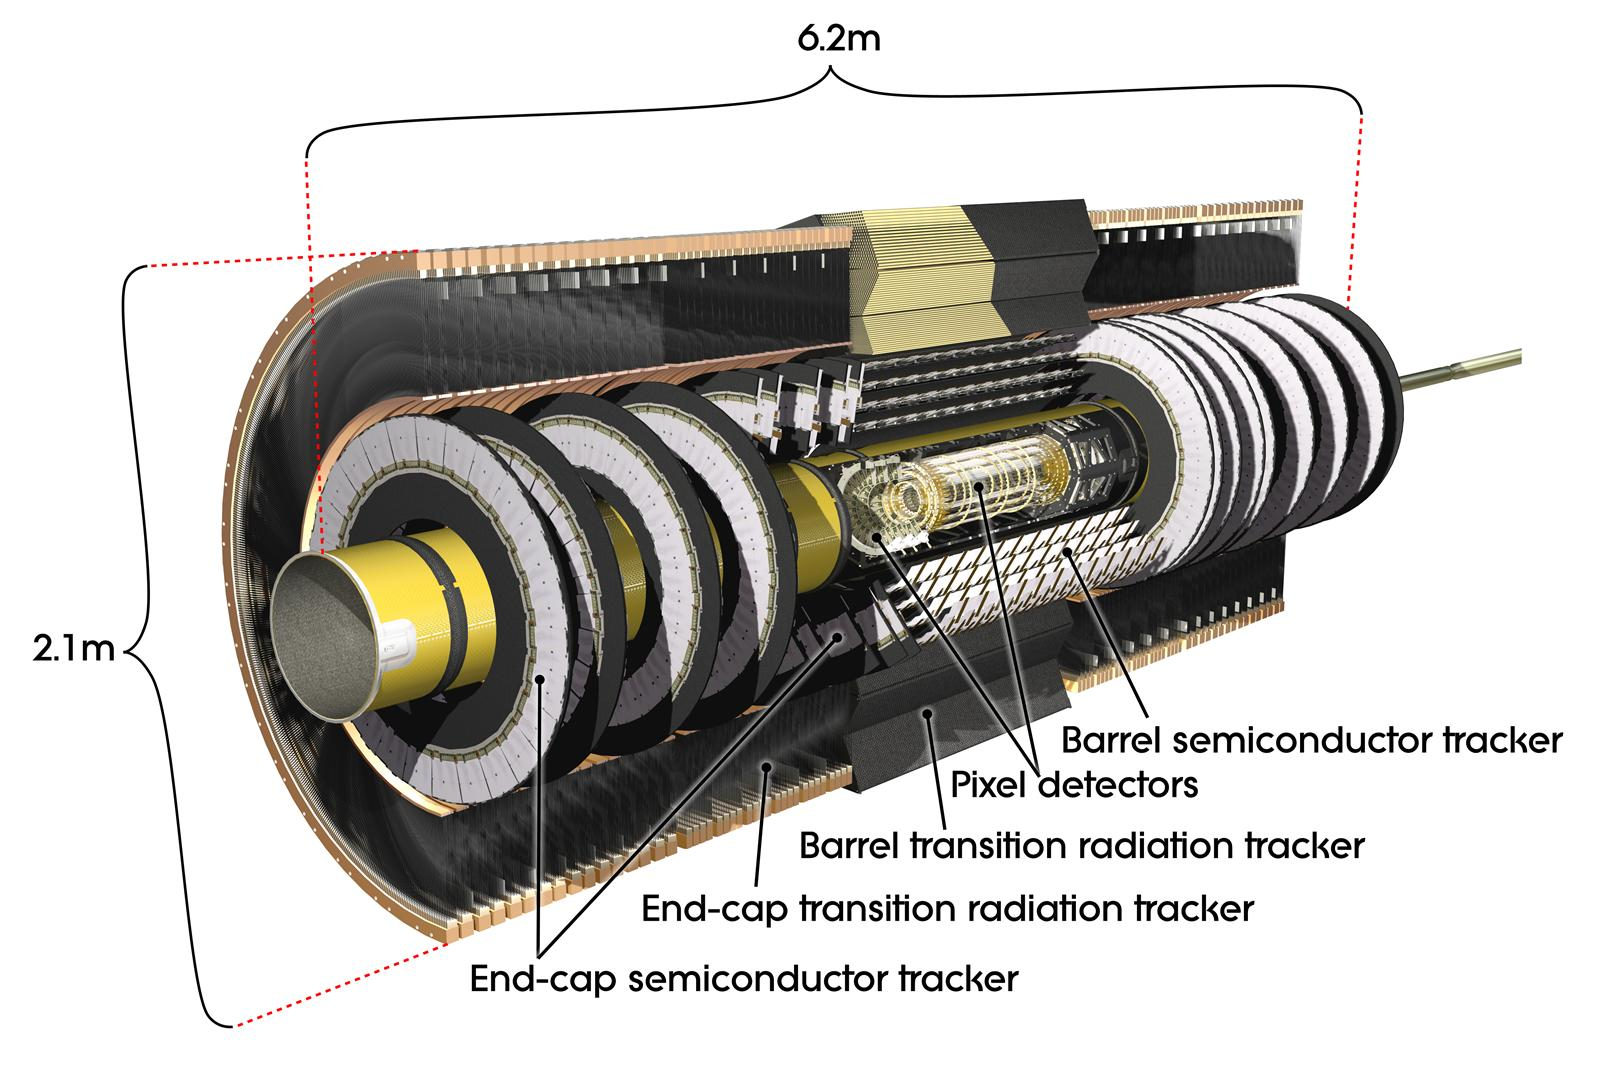
\includegraphics[width=0.8\textwidth]{images/lhc/pixel_2.jpg}
  \caption{Esquema del detector interno de ATLAS \cite{Pequenao:1095926}.}
  % https://cds.cern.ch/record/1095926
  \label{fig:pixel_1}
\end{figure}

\begin{figure}
  \centering
  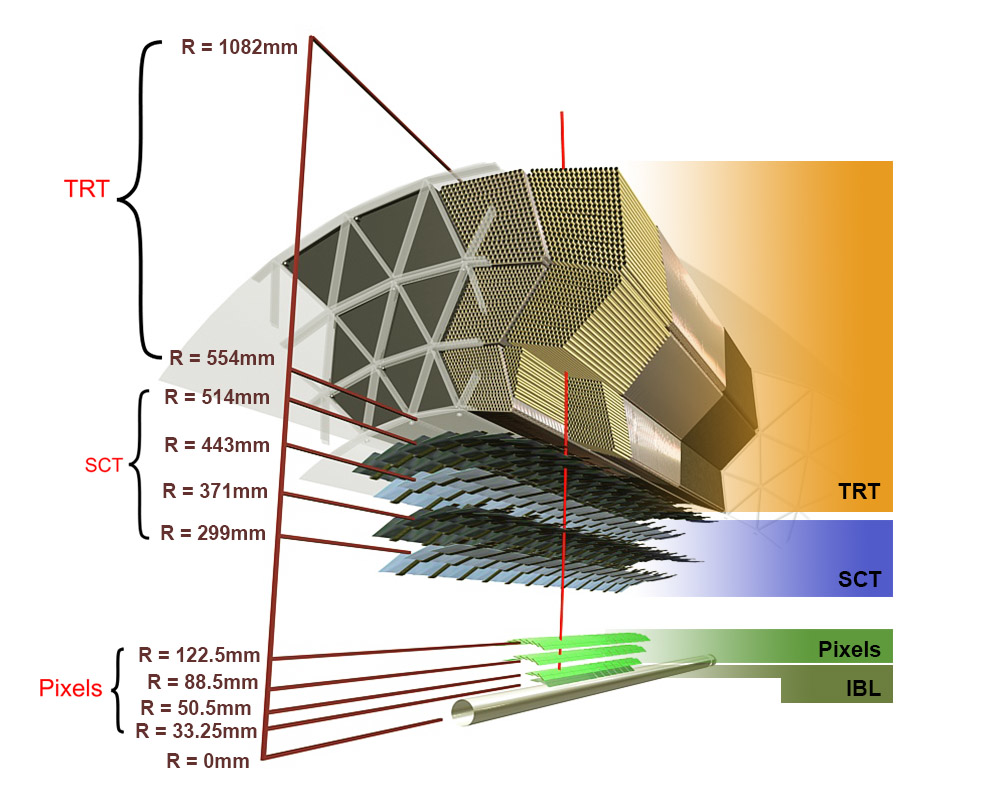
\includegraphics[width=0.45\textwidth]{images/lhc/pixel_1.png}
  % https://cds.cern.ch/record/2724037
  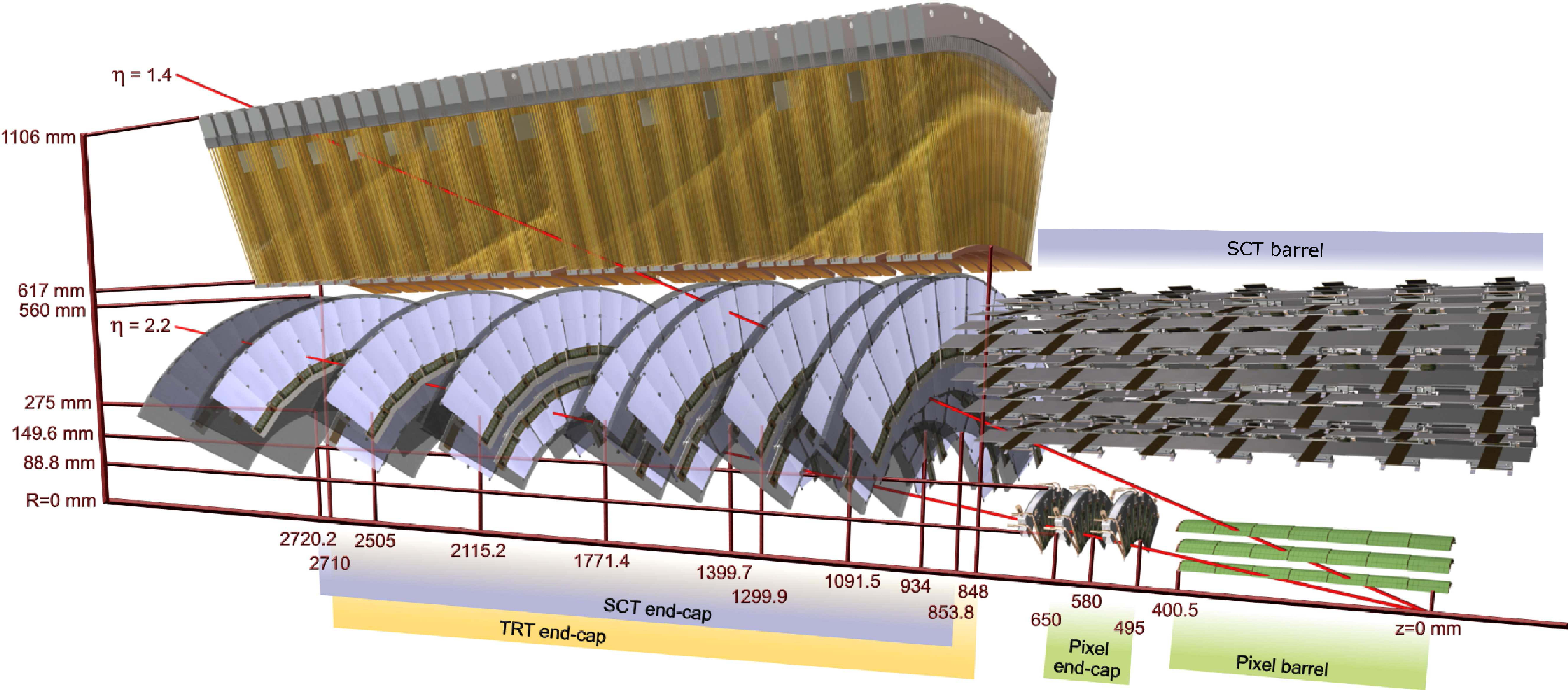
\includegraphics[width=0.55\textwidth]{images/lhc/pixel_4.png}
  % https://cds.cern.ch/record/1298112
  \caption{Diferentes vistas del detector interno de ATLAS \cite{Pequenao:1095926,Kayl:1298112}.}
  \label{fig:pixel_23}
\end{figure}


\subsubsection{Detector de píxeles}

El detector de píxeles fue construido para medir la posición de las trazas de partículas cargadas con la más alta precisión posible y es de vital importancia para la reconstrucción de los vértices primarios y secundarios. En la región barrel el detector se compone de tres capas cilíndricas, mientras que la endcap de tres discos. La capa más interna, denominada \textit{InsertableB-Layer} (IBL) \cite{ATLAS-TDR-2010-19}, se encuentra a \magn{50.5}{mm} del punto de interacción.
El principio de detección para partículas cargadas es la medida de la deposición de la carga inducida en una capa de silicio por ionización. El sistema contiene un total de $80$ millones de sensores, cada uno con una resolución de \magn{10}{$\mu$m} ($R-\phi$) y \magn{115}{$\mu$m} ($z$). Estos módulos en la región barrel, se encuentran levemente solapados y rotados para proveer una cobertura total en el ángulo azimutal. La Figura \ref{fig:pixel_3} muestra un esquema completo del detector de píxeles.

La inclusión del IBL fue una de las actualizaciones del Run 2 motivada por el incremento de luminosidad del LHC, lo que podía significar un daño por radiación en los detectores internos. En vez de reemplazar las partes del detector de píxeles que podían ser dañadas, se decidió colocar una capa adicional entre el detector de píxeles y la tubería donde circulan los protones. El objetivo del mismo es mejorar la eficiencia en la identificación de trazas, vértices, y en la identificación de bottom quarks, que decaen típicamente fuera del radio del IBL. El IBL está compuesto por $8$ millones de chips de rápida lectura y con sensores de silicio, que detectan el paso de partículas cargadas mediante la deposición de carga inducida. El tamaño de los píxeles es de $50\times250\,\mu$m$^{2}$, con una resolución de \magn{8}{$\mu$m} ($R-\phi$) y \magn{40}{$\mu$m} ($z$). La distancia entre el IBL y la tubería es de \magn{0.2}{mm}, y entre el tubo y el detector de píxeles es de \magn{1.9}{mm}. 


\begin{figure}
  \centering
  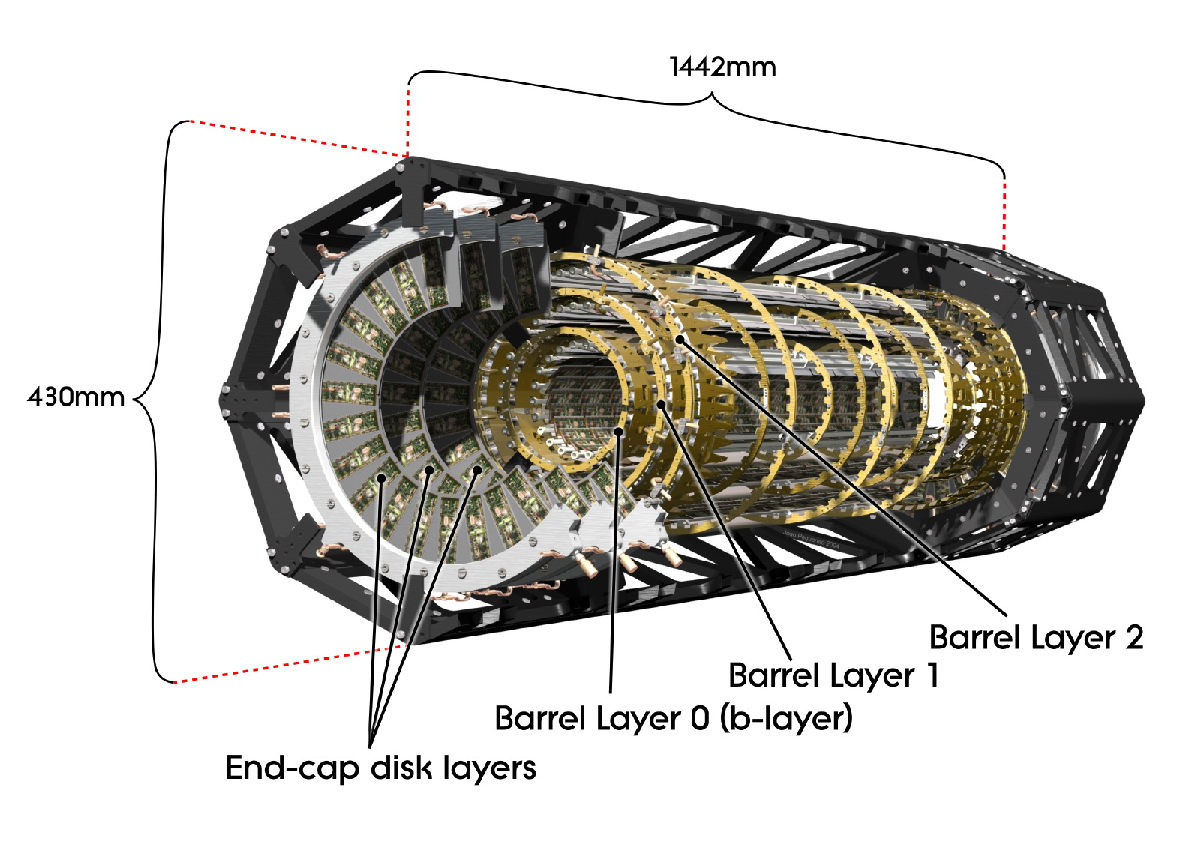
\includegraphics[width=0.7\textwidth]{images/lhc/pixel_3.png}
  % https://cds.cern.ch/record/1957197
  \caption{Esquema del detector de píxeles de ATLAS \cite{Takubo:1957197}.}
  \label{fig:pixel_3}
\end{figure}

\subsubsection{Detector Semiconductor de Trazas (SCT)}

Se encuentra por fuera del detector de píxeles y está diseñado para medir las trazas con alta precisión en la zona intermedia del detector. A diferencia del detector de píxeles, estos sensores de silicio están segmentados en micro bandas, dado que es más baja multiplicidad de partículas es posible reducir la resolución al costo de aumentar el área de cobertura. La resolución de \magn{17}{$\mu$m} ($R-\phi$) y \magn{580}{$\mu$m} ($z$). En la región barrel los módulos de SCT están dispuestos en cuatro capas concéntricas, y levemente solapados y rotados para proveer una cobertura total en el ángulo azimutal. La región endcap consiste en nueve discos transversales al eje del haz.


\subsubsection{Detector de Radiación de Transición (TRT)}

Es el detector más externo del ID y está diseñado, no solo para detectar partículas cargadas, sino también para distinguir entre partículas pesadas y livianas. El TRT se compone de tubos detectores de \magn{4}{mm} de diámetro, con un gas que se ioniza al ser atravesado por partículas cargadas. Los electrones producidos son colectados por una ánodo, y el tiempo de deriva es una medida de la distancia a la traza del mismo. Además, los tubos están rodeados de fibras de polipropileno con un índice de refracción diferente, por lo que las partículas que atraviesan el detector emiten radiación con una intensidad proporcional a $\gamma=E/m$, permitiendo al TRT  distinguir partículas cargadas pesadas ($\pi^{\pm}$) de aquellas más livianas ($e^{\pm}$). La región barrel contiene $50000$ tubos paralelos al eje del haz y la región endcap $320000$ tubos orientados radialmente, cuya resolución es de \magn{0.17}{mm}.

\subsection{Calorímetros}


El sistema de calorímetros de ATLAS está diseñado para medir la energía y la posición de las partículas, mediante la absorción de la energía depositada por las cascadas de partículas secundarias que estas generan en el material del mismo. Además, permite discriminar entre jets producidos por quarks o gluones de los electrones y fotones, detectar aquellas partículas neutras que no dejaron trazas en el ID y realizar la selección online de eventos potencialmente interesantes (Ver Sistema de trigger). Gracias a su amplia cobertura y a que absorbe la energía de prácticamente todas las partículas producidas (salvo muones) es de gran utilidad para poder medir el desbalance de energía transversa, magnitud discriminatoria utilizada en la mayoría de análisis fuera del SM.

Está compuesto de un calorímetro electromagnético (ECAL) dedicado principalmente a la medida de las deposiciones de partículas como fotones y electrones (partículas interactuantes principalmente vía interacción EM), y otro hadrónico (HCAL) dedicado a las cascadas de partículas producto de la hadronización de los quarks o gluones (jets) (partículas interactuantes principalmente vía interacción fuerte). La Figura \ref{fig:calo_1} muestra un esquema de los calorímetros del detector ATLAS.

\begin{figure}
\centering
  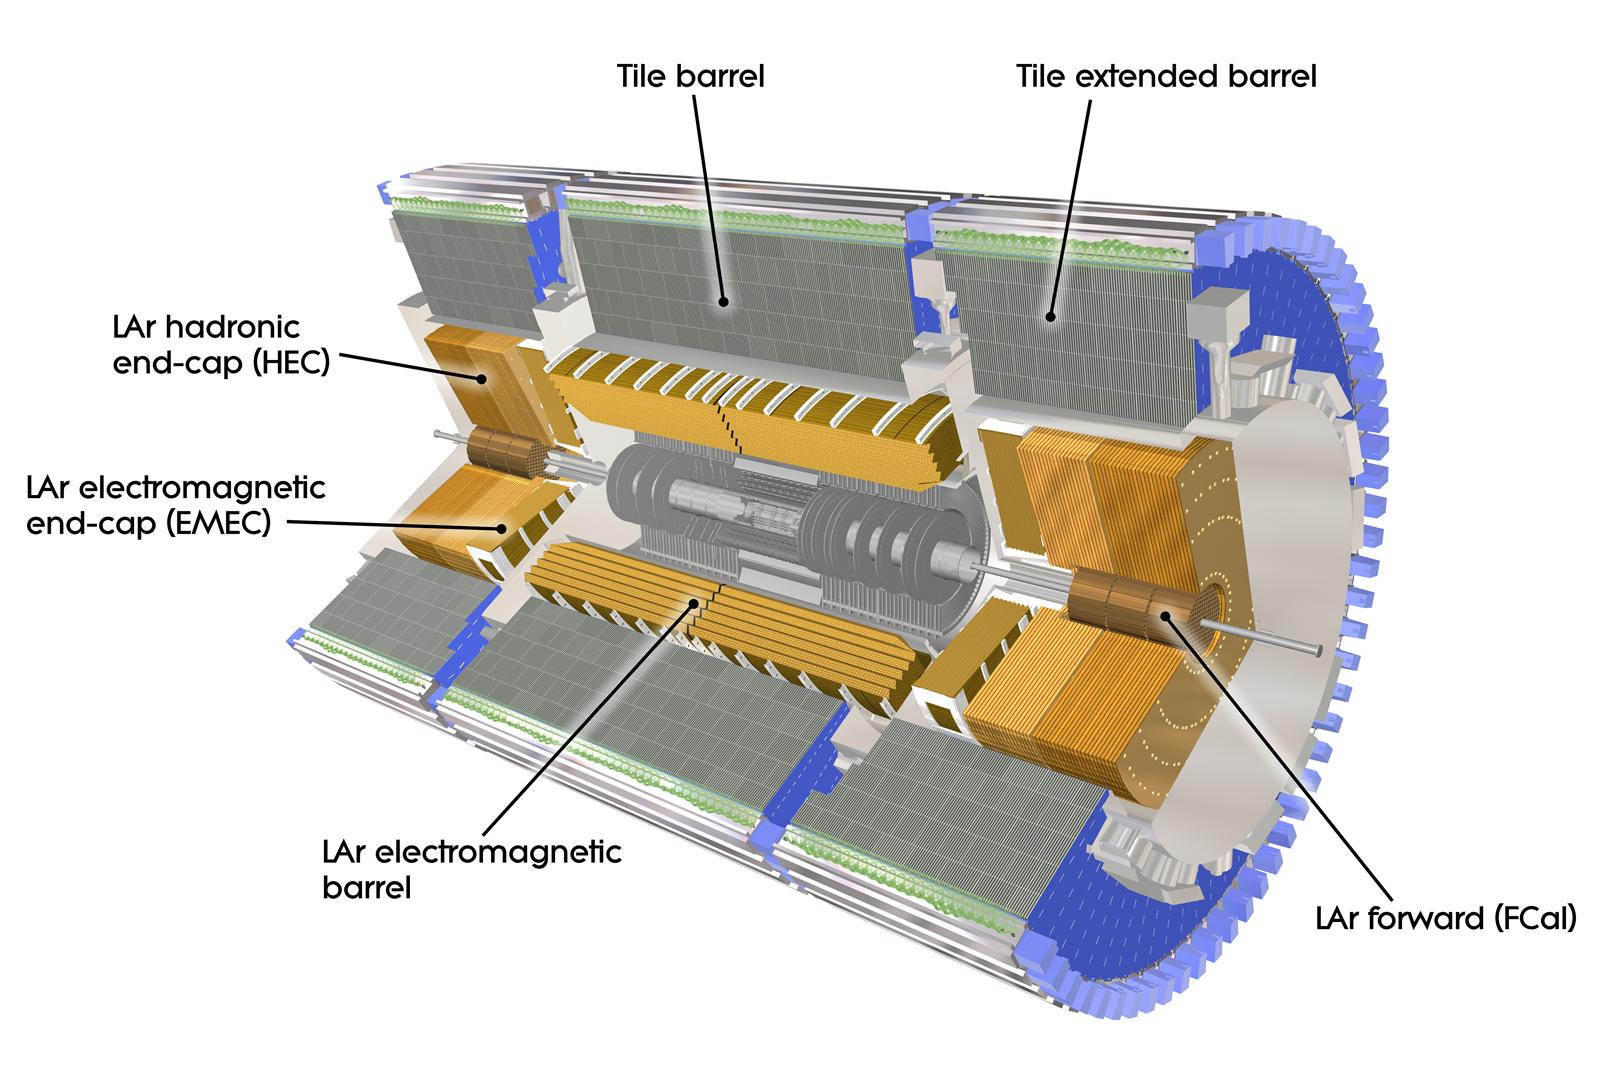
\includegraphics[width=0.7\textwidth]{images/lhc/calo_1.jpg}
  % https://cds.cern.ch/record/1095927 calo_1.png
  % https://cds.cern.ch/record/2239809 calo_2.png
  \caption{Esquema de los calorímetros del detector ATLAS \cite{Pequenao:1095927}.}
  \label{fig:calo_1}
\end{figure}

\subsubsection{Calorímetro electromagnético (ECAL)}

El ECAL en un calorímetro de muestreo (inhomogéneo) no compensado, que utiliza plomo como material absorbente y argón líquido como material absorbente. Consiste en varias placas de plomo dispuestas en forma de acordeón que se colocan de forma alterna inmersas en LAr. Las partículas incidentes interactúan con el Plomo creando una lluvia de partículas cargadas y neutras. Las partículas cargadas ionizan el medio activo, donde los electrones liberados son colectados en un electrodo central de kaptón/cobre hacia donde derivan por acción del campo eléctrico aplicado. La señal total en el medio activo es así proporcional a la energía total real de la partícula incidente. La ventaja de este método es la detalla reconstrucción de la forma de la cascada, al costo de no poder reconstruir la totalidad de la energía de la cascada debido al espacio que existe entre placa y placa.


El ECAL está dividido en dos mitades dentro de la región barrel ($\eta < 1.475$) y en dos componentes (una a cada lado) en la región endcap ($1.375 < |\eta| < 3.2$). 
En la región de transición \footnote{Denominada también como región \textit{crack}.} entre el barrel y el endcap, comprendida entre $1.37 < |\eta| < 1.52$, se encuentra una zona no instrumentada donde se encuentra el cableado del detector. 
Allí naturalmente la calidad de detección es menor, y es por ese motivo que la mayoría de los análisis excluye a los candidatos a fotones o electrones que estén reconstruidos en esta región.

En la región diseñada para medidas de precisión ($\eta < 2.5$, excluyendo el crack),
el ECAL está segmentado en tres capas longitudinales. La primera capa consiste de
bandas con fina granularidad (en la dirección de $\eta$), para discriminar entre fotones
aislados y pares de fotones espacialmente cercanos provenientes del decaimiento
$\pi^0\to\gamma\gamma$. Para los electrones y fotones con alta energía transversa, la mayoría
de la energía se colecta en la segunda capa, que tiene una granularidad lateral de
$0.025 \times 0.025$ en $(\eta, \phi)$. La tercer capa se encarga de la energía depositada en las
colas de la lluvia.
El espesor del ECAL es mayor a 22 longitudes de radiación ($X_0$) en la región
barrel, y mayor a 24 $X_0$ en los endcap, donde una longitud de radiación se define
como la distancia promedio sobre la cual la energía de un electrón se reduce a $1/e$
de su energía inicial. Para el caso de los fotones, una reducción similar se obtiene a
$9/7$ de $X_0$ . Por tanto, toda la energía electromagnética es absorbida en el ECAL y
sólo parte de la componente hadrónica llega al HCAL. En la Figura \ref{fig:ecal} se observa un segmento del ECAL donde se muestra la granularidad de cada una de sus capas.

\begin{figure}
\centering
  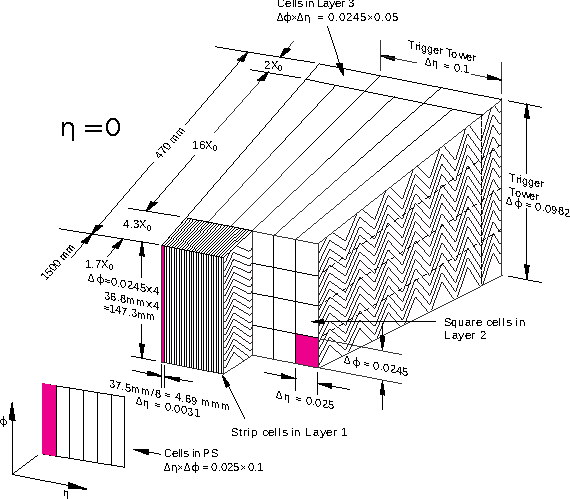
\includegraphics[width=0.7\textwidth]{images/lhc/ecal.pdf}
  \caption{Segmento del ECAL del detector ATLAS en la región con $\eta=0$ \cite{PERF-2017-01}.}
  \label{fig:ecal}
\end{figure}

\subsubsection{Calorímetro hadrónico (HCAL)}

El HCAL es un conjunto de calorímetros que rodean al ECAL, extendiendo la aceptancia del calorímetro de ATLAS hasta cubrir prácticamente la totalidad de ángulo sólido del punto de colisión.

El primero de los calorímetros se denomina \textit{Tile Calorimeter}, es un calorímetro de muestreo que utiliza acero como material absorbente y tejas centelladoras plásticas como material activo, se encuentra en la región barrel y está dividido en dos partes que tienen una cobertura de $|\eta|<1.0$ y $0.8<|\eta|<1.7$ respectivamente. Los centelladores, dispuesto en un arreglo
periódico, se conectan a una fibra óptica que trasporta la luz producida por el paso
de partículas, hacia un tubo fotomultiplicador. Este arreglo se extiende radialmente, de los
\magn{2.28}{m} a los \magn{4.25}{m}. 
En la región endcap se encuentra un calorímetro hadrónico de muestreo (HEC) con placas de cobre como absorbente y argón líquido como material activo, que consiste en dos ruedas, una atrás de la otra con las placas planas de cobre dispuestas perpendicularmente al eje del haz, con un radio de 2.3\ m. Finalmente se encuentra el \textit{Forward Calorimeter} (FCAL), un calorímetro de muestreo que extiende la cobertura del sistema a $|\eta|<4.9$, coaxial
al eje del haz y ubicado a \magn{4.7}{m} a cada lado del punto de interacción. El material
principal de los módulos es argón líquido (con cobre o tungsteno), y si bien no se
utiliza para mediciones de precisión, provee información para el cómputo de la energía transversa faltante y la reconstrucción de jets en regiones muy cercanas al eje
del haz.



Por su parte, el HCAL tiene un espesor mayor a $7.7$ longitudes de interacción
hadrónica ($\lambda$) en la región barrel ($9.7\lambda$ en total si se cuenta el ECAL). De manera
análoga a la longitud de radiación mencionada para el ECAL, una longitud de
interacción hadrónica se define como la distancia promedio sobre la cual la energía
de un hadrón se reduce a $1/e$ de su energía inicial. De esta forma, toda la energía
con la que llegan los hadrones al HCAL, queda allí depositada.

\subsection{Espectrómetro de muones}

El espectrómetro de muones (MS) se encuentra situado en la parte más externa del detector ATLAS. Esto se debe a que los muones de alto \pt generados en el punto de interacción tienen un altísimo poder de penetración y son poco interactuantes, siendo las únicas partículas detectables capaces de llegar a este detector. El mismo se encuentra intercalado con el sistema de imanes toroidales, y está diseñado para obtener mediciones de alta precisión de la posición e impulso de los muones, y para una rápida identificación para el sistema de trigger. Este es el subdetector más grande y el que le da a ATLAS su tamaño característico. 

El MS se compone de diferentes tipos de cámaras de detección de muones (ver Figura \ref{fig:muon_1}). Las \textit{Monitored Drift Tubes} (MDTs) son responsables de la mayoría de las medidas de precisión y cubren el rango de $|\eta|<2.7$. Funcionan de forma similar al TRT, con tubos llenos de un gas que ioniza y un ánodo central que recoge los electrones producidos, y el tiempo de deriva se asocia con la distancia a la traza. En la región endcap se encuentran las \textit{Cathode Strip Chambers} (CSCs) que poseen alta resolución espacio-temporal y una cobertura $|\eta|>2.0$. Estas cámaras funcionan midiendo la carga depositada en un ánodo, producto de la cascada de electrones creados cerca del mismo. Las \textit{Resistive Plate Chamber} (RPCs) proveen una estimación rápida del momento de los muones al primer nivel del trigger con una cobertura de $|\eta|<1.05$. Las RPCs miden la descarga ocasionada entre dos placas resistivas paralelas sometidas a una alta diferencia de potencial, tras la ionización del volumen de gas interno causada por el paso de muones energéticos. Finalmente se encuentra en la región endcap las \textit{Thin Gap Chambers} (TGCs), similares en funcionamiento a las CSCs. Proveen también información al sistema de trigger en esta región y tienen una cobertura de $|\eta|<2.4$.

\begin{figure}
  \centering
  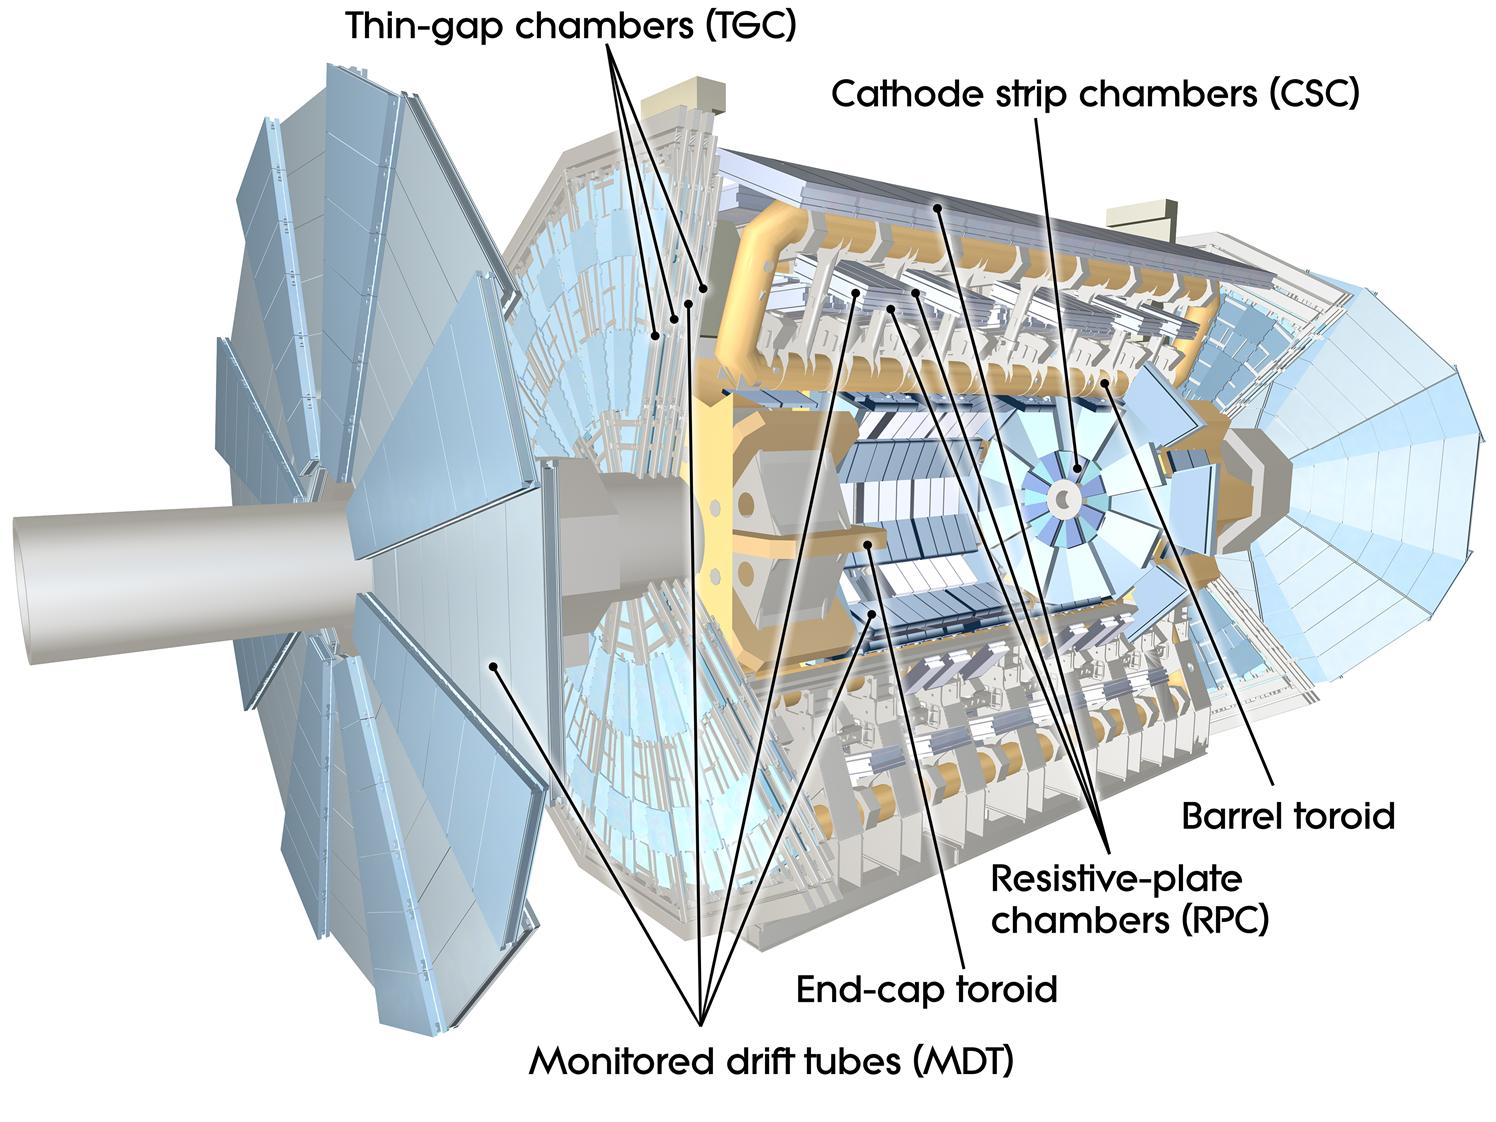
\includegraphics[width=0.7\textwidth]{images/lhc/muon_1.jpg}
  \caption{Espetrómetro de muones del detector ATLAS \cite{Pequenao:1095929}.}
  % https://cds.cern.ch/record/1095929
  \label{fig:muon_1}
\end{figure}

\section{Sistema de \textit{trigger}}
\label{trigger}

Como se mencionó anteriormente, el diseño del LHC permite tener una frecuencia de cruces de paquetes de 40 MHz y del orden de 30 interacciones promedio por cruce de paquetes ($\langle \mu \rangle$), lo que da una tasa de interacción protón-protón del orden del GHz. Tal frecuencia requeriría un ancho de banda de escritura y una la capacidad de almacenamiento excesivos. De todas formas, no todos los eventos son de interés para la colaboración, como por ejemplo la colisión elástica de los protones que no genera ningún tipo de decaimiento. El sistema de trigger del detector ATLAS \cite{TRIG-2016-01} es el encargado de filtrar esos eventos de poco interés y, junto con el sistema de adquisición de datos (DAQ), almacena aquellos que potencialmente pueden llegar a ser de interés para los distintos análisis, reduciendo así la frecuencia de flujo de datos al orden del kHz. El sistema de trigger cumple un rol central en el correcto funcionamiento de todo el experimento, ya que en definitiva determina qué tipos de análisis se realizarán y qué nueva física podrá encontrarse. El mismo debe tener una alta eficiencia, para no desechar eventos importantes, pero con el compromiso de mantener el flujo de datos relativamente bajo. 

El sistema de trigger está compuesto por dos niveles consecutivos capaces de realizar una identificación de partículas cada vez más compleja: un primer nivel de trigger (L1) basado en hardware y luego un trigger de alto nivel basado en software (HLT). La Figura \ref{tdaq} muestra un esquema del sistema trigger y DAQ del detector ATLAS. Una secuencia de algoritmos del L1 y del HLT se denomina cadena de trigger \footnote{En inglés \textit{Trigger chain}, pero también dentro de la jerga se las puede llamar simplemente triggers}, que impone requisitos sobre las características de los objetos presentes en el evento y a partir de ellas decide si el evento es aceptado. El conjunto de cadenas de triggers que se emplea durante la toma de datos se denomina \textit{Trigger menu}, que se optimiza previamente para satisfacer las condiciones del LHC sin afectar la adquisición de datos. Para controlar la tasa de eventos aceptados, a algunos triggers se les asigna un valor denominado \textit{prescale}, el cual puede estar tanto en el L1 como en el HLT. Para un prescale de valor $n$, el evento tiene una probabilidad $1/n$ de ser aceptado por dicho trigger. El valor del prescale puede ser mayor a uno, reduciendo así la tasa de eventos aceptados (inclusive anulándola por completo), o igual a uno (`sin prescale' o \textit{unprescaled}). En este caso todos los eventos son evaluados, y se emplea en general para los triggers principales orientados para su uso en análisis físicos. El prescale es modificado de acuerdo a la luminosidad durante una toma de datos, para mantener la tasa de datos constante, sin saturar el ancho de banda. Para el caso de los triggers con prescale o aquellos directamente deshabilitados, se los puede configurar en un modo denominado \textit{rerun}, para el cual los algoritmos del trigger se corren offline una vez que el evento fue aceptado por otro trigger. A continuación se describen los dos niveles que componen al sistema de trigger.

\begin{figure}
  \centering
  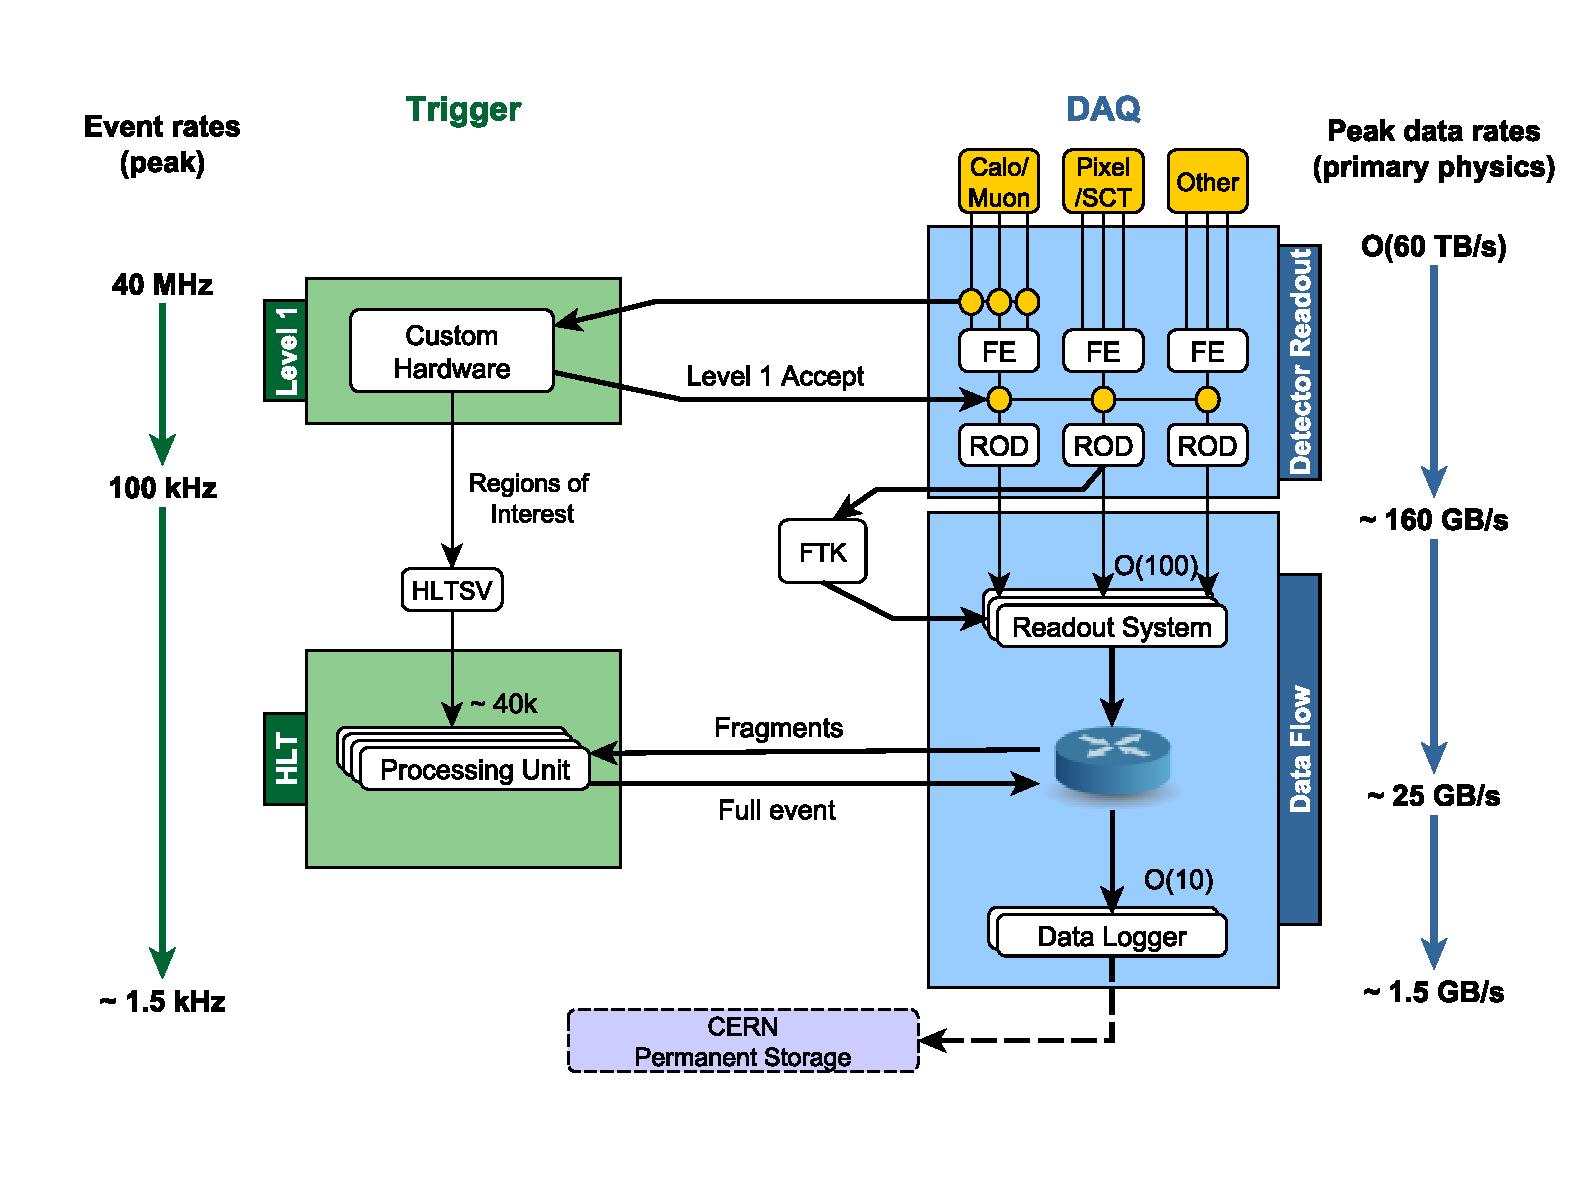
\includegraphics[width=0.7\textwidth]{images/lhc/tdaqFullNew2017.pdf}
  % https://twiki.cern.ch/twiki/pub/AtlasPublic/ApprovedPlotsDAQ/tdaqFullNew2017.png
  \caption{Esquema del sistema de trigger y el sistema de adquisición de datos de ATLAS \cite{tdaq_plot}.}
  \label{tdaq}
\end{figure}

\subsubsection{Level 1 (L1)}

El primer nivel del trigger \cite{level1} está basado en hardware, y reduce los 40 MHz del LHC a menos de \magn{100}{kHz} con una latencia de aproximadamente \magn{2.5}{$\mu$s}, tiempo determinado por el limitado tamaño de los \textit{buffers} de memoria y por el tiempo que le toma a los muones producidos en el evento alcanzar el MS. Utiliza la información recolectada en una región reducida (capas) del calorímetro y del MS, para así reconstruir lo que se denominan Regiones de Interés (RoI). Las RoIs se determinan por la posición de la deposición de energía en el calorímetro por parte de las partículas consideradas de interés (en el caso de los muones es en el MS), permitiendo una rápida reconstrucción de su energía transversa, y aplicando un posible filtro en esta magnitud. El diseño del L1 permite tener una aceptancia en el rango de $|\eta|<2.5$ para electrones, fotones, muones y taus, hasta $|\eta|<3.2$ para jets, y $|\eta|<4.9$ para el cálculo del momento transverso faltante. Las RoIs a su vez sirven como semilla para el HLT que realiza selecciones más detalladas a partir de las mismas.

\subsubsection{High Level Trigger (HLT)}

Cuando un evento es aceptado por el L1, el mismo pasa a ser analizado por High Level Trigger \cite{ATLAS-TDR-16}, que está basado en software y permite reducir la tasa de eventos que se almacena a \magn{1.5}{kHz} con una latencia de \magn{0.2}{s}. El mismo utiliza las RoIs previamente reconstruidas por el L1, y ejecuta una secuencia de algoritmos aplicados sobre el objeto candidato. Si uno de los pasos de la secuencia falla en los requisitos, los siguientes pasos no son aplicados para ahorrar tiempo de cómputo. 


Los algoritmos del HLT constan de dos etapas: los algoritmos de reconstrucción rápida ejecutados primero, y luego los algoritmos de reconstrucción de precisión similar a los que se utilizan en la selección offline. Los algoritmos de reconstrucción rápida utilizan la información de los calorímetros y de las trazas sólo dentro de la RoI para realizar la selección e identificación de los candidatos, y realizar el rechazo de fondo lo más rápido y temprano posible. Si la partícula candidata pasa los criterios definidos por la selección de reconstrucción rápida, se ejecutan los algoritmos de selección de precisión. Estos tienen acceso a la información del detector fuera de la RoI, con la máxima granularidad e incluyendo detalles sobre la calibración de energía de los calorímetros, la alineación de los subdetectores y el mapa de campo magnético. Los eventos aceptados por el HLT son finalmente grabados a disco y distribuidos, accesibles offline para todos los diferentes estudios y análisis.

% \tosolve{Definir pileup, prescale y rerun} Done!

\section{Modelo computacional y distribución de datos}\label{sec:lhc_samples}

% esta igual a la tesis de joaco, arreglar: Done!!! Searching for Dark Matter with the ATLAS Detector, Steven Schramm

La enorme cantidad de datos tanto producidos por las colisiones en el LHC ($\sim$\,PB al año), como por las simulaciones de MC requiere un sistema de cómputo de alta complejidad, que permita el acceso de los mismos a todos los miembros de la colaboración de una manera ágil y directa. Esto se logra mediante la \textit{Worldwide LHC Computing Grid} (WLCG), la cual comparte el poder de procesamiento y la capacidad de almacenamiento entre distintos centros de cómputo distribuidos alrededor del mundo (\textit{Tiers}). Todos los eventos son inicialmente almacenados en el Tier 0 del CERN, el cual contiene el 20\% de cal capacidad de cómputo total del WLCG. A medida que se van procesando esos datos y reduciendo su tamaño, se van repartiendo entre acorde los Tier 1, 2 y 3.

Inicialmente los eventos aceptados por el HLT son almacenados como \textit{Raw Data Objects} (RDOs), los cuales contienen una enorme cantidad de información del detector. Esta información es de poca utilidad para los usuarios, y por ende es procesada en distintos formatos que contienen los objetos finales útiles para los análisis. Para ello se aplican distintos criterios de \textit{sliming} (se remueven los eventos que no son de interés), \textit{skiming} (se remueve la información irrelevante de los objetos) y \textit{thining} (se remueven objetos y/o colecciones de objetos irrelevantes) según los estudios y análisis que se vayan a realizar sobre los datos colectados. Los RDOs son empleados para la reconstrucción y calibración de objetos físicos, que se almacenan en el formato \textit{Event Summary Data} (ESD). Adicionalmente se realiza un procesamiento el cual descarta la mayoría de la información de las celdas, generando el formato \textit{Analysis Object Data} (AOD), el cual tiene un tamaño de $\sim$100\,kB por evento. Para el Run 2, se empleó un formato adicional (\texttt{xAOD}) que reducía significativamente este formato (10-15\,kB por evento). Estos últimos formatos son archivos accesibles vía el entorno de análisis de datos \texttt{ROOT} \cite{root}, que contienen el conjunto de  objetos físicos finales reconstruidos, y son empleados por los usuarios para realizar los distintos análisis.
El software de ATLAS se desarrolla dentro un entorno \texttt{C++} común llamado \texttt{ATHENA} \cite{ATLAS-TDR-17, analysistools, athena}, en el que se realiza todo el procesamiento de datos. 

Adicionalmente se puede aplicar una selección a los eventos de las \texttt{xAOD} para reducir aún más su tamaño. Esta selección produce el formato \textit{Derived Analysis Objetc Data} (DAOD), o simplemente derivación, y existen varias dependiendo de la selección empleada por cada análisis. Las derivaciones de interés para esta tesis son las denominadas \texttt{EGAM3}, \texttt{EGAM4} y \texttt{SUSY1}. Las \texttt{EGAM3} y \texttt{EGAM4} son utilizadas en esta tesis para la medida de la eficiencia de los trigger de fotones, ya que preseleccionan eventos con bosones $Z$ decayendo radiativamente a partir de electrones o muones respectivamente. La derivación \texttt{SUSY1} es utilizada en esta tesis para preseleccionar los eventos para la búsqueda de supersimetría, y en general selecciona eventos con objetos energéticos. A continuación se lista un resumen de las selecciones que deben cumplir los eventos para ser aceptados por estas derivaciones:


\begin{itemize}
  \item \texttt{EGAM3}: El evento debe tener al menos dos electrones de carga opuesta y un fotón, en general con $\pt>9.5\,\gev$. Este último requisito varía dependiendo de los criterios de calidad de los electrones. A su vez se solicita una masa invariante de los leptones mayor a \magn{40}{GeV}.
  \item \texttt{EGAM4}: Similar a \texttt{EGAM3} pero seleccionando muones en vez de electrones.
  \item \texttt{SUSY1}: Selecciona eventos con jets o fotones cuya suma de momentos transversos supere los \magn{150}{GeV}. A su vez selecciona eventos con al menos un electrón, muón o fotón con $\pt>100\, \gev$, o al menos dos electrones o muones con $\pt>20\,\gev$, o al menos menos dos fotones con $\pt>50\, \gev$.
\end{itemize}

% \subsubsection{\texttt{EGAM3}}
% \begin{itemize}

%   \item Dos electrones centrales de carga opuesta, con identificación medium o LLHmedium, con $\pt>9.5$ GeV y masa invariante de ambos mayor a $40$ GeV, más un fotón con $\ET>9.5$ GeV.

%   \item Selección anterior, pero reemplazando el fotón por un electrón central.

%   \item Dos electrones centrales de carga opuesta, al menos uno con identificación tight o LHH tight y $\pt>24.5$ GeV, el otro con $\pt>6.5$ GeV y masa invariante de ambos mayor a $40$ GeV, más un fotón tight con $\ET>9.5$ GeV.

%   \item Dos electrones de carga opuesta, uno central tight o LLHtight, $\pt>24.5$ GeV, el otro forward con $\pt>6.5$ GeV y masa invariante de ambos mayor a $40$ GeV, más un fotón tight con $\ET>9.5 GeV$ 

% \end{itemize}

% \subsubsection{\texttt{EGAM4}}
% \begin{itemize}

%   \item Al menos dos muones de carga opuesta 'commongood' con $\pt>9.5$ GeV, $|\eta|<2.7$ y masa invariante de ambos mayor a $40$ GeV, más un fotón con $\ET>9.5$ GeV.

%   \item Selección anterior, pero reemplazando el fotón por un electrón central.

%   \item Al menos dos electrones centrales de signo opuesto, al menos uno con identificación tight o LHH tight y $\pt>24.5$ GeV, el otro con $\pt>6.5$ GeV y masa invariante de ambos mayor a $40$ GeV, más un fotón tight con $\ET>9.5$ GeV.

%   \item Al menos dos electrones de signo opuesto, uno central tight o LLHtight, $\pt>24.5$ GeV, el otro forward con $\pt>6.5$ GeV y masa invariante de ambos mayor a $40$ GeV, más un electrón con $\pt>9.5 GeV$ 

% \end{itemize}

% \subsubsection{\texttt{SUSY1}}
% \begin{itemize}

%   \item $\HT>150$ GeV
%   \item Al menos un electrón, muón o fotón con $\pt>100$ GeV
%   \item Al menos dos electrones o muones con $\pt>20$ GeV
%   \item Al menos dos fotones con $\pt>50$ GeV

% \end{itemize}


\section{Simulaciones de Monte Carlo}

% principalmente de la tesis de joaco: solucionado!!!

El método de Monte Carlo utiliza una serie de algoritmos computacionales basados en la repetición de eventos con un factor variable y aleatorio, que permite obtener resultados numéricos globales.
En el contexto de la física de partículas no solo se utiliza para reproducir la aleatoriedad impuesta por la mecánica cuántica, sino también para realizar diferentes aproximaciones, como es el caso de integrales numéricas.
Las simulaciones de Monte Carlo cumplen un rol fundamental a la hora de realizar predicciones de la teoría, teniendo un rol primordial en prácticamente todos los análisis realizados por la colaboración ATLAS. 

Las simulaciones de colisiones de protones se realizan a partir de complejos cálculos basados en la teoría de QCD y descriptas brevemente en la Sección \ref{sec:qcd_pp}. 
El punto central de la simulación es la dispersión dura (\textit{Hard Scatter}, HS) que se calcula a un dado orden de la teoría de perturbaciones. Para ello se emplean programas generadores de elementos de matriz (ME), las cuales contienen  la información de la función de onda para los partones entrantes y salientes, y depende principalmente del acoplamiento
fuerte y la escala de energía de la dispersión. La evolución de los partones producidos se realiza mediante un modelo de lluvia de partones (\textit{Parton Shower}, PS) que conecta la escala dura de los partones de color, con la escala de la hadronización donde se generan los hadrones de color, y es el límite de validez del régimen perturbativo $\Lambda_{\text{QCD}}\sim 1$\,GeV. En esta etapa los partones son transformados en hadrones primarios aplicando modelos de fragmentación puramente fenomenológicos, generando así una cascada de partículas formada por un gran número de gluones y quarks de baja energía. La combinación entre la dispersión dura y la lluvia partónica debe realizarse
con especial cuidado de no duplicar en la PS los partones ya producidos y evitar
así el doble conteo. Las estrategias principales para esto se conocen como CKKW
(Catani-Krauss-Kuhn-Webber) \cite{ckkw_1, ckkw_2} y MLM \cite{mlm}. Finalmente los hadrones son decaídos en partículas estables que son las que observa el detector.

Adicional al HS existen otros procesos QCD que ocurren en la colisión. Debido a que los quarks son cargados bajo QCD y los gluones tienen acoplamientos triples y cuádruples, puede suceder que los partones emitan quarks o gluones antes de la dispersión dura (\textit{Initial State Radiation}, ISR). De manera análoga, los partones salientes pueden emitir gluones o
producir pares de quarks/anti-quarks (\textit{Final State Radiation}, FSR). A su vez, pueden darse interacciones adicionales entre partones pertenecientes a los protones originales, que no participaron de la dispersión dura, dando lugar a múltiples
interacciones en el evento, mayoritariamente interacciones de bajo momento. La actividad no asociada con la dispersión dura se llama evento subyacente
(\textit{Underlying Event}, UE), que debido a la baja energía de las interacciones que lo
componen, no puede ser tratado de manera perturbativa y se requieren de modelos
fenomenológicos para describirlos. En la Figura \ref{fig:mc_qcd} se puede observar el diagrama de una colisión entre partones, junto con la cascada de partículas producto de la misma.

\begin{figure}
  \centering
  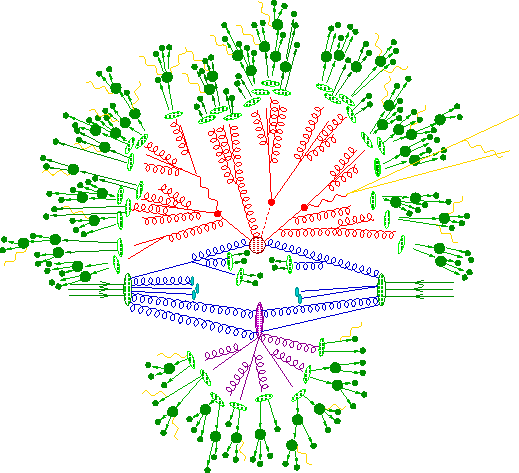
\includegraphics[width=0.8\textwidth]{images/lhc/mc_qcd.pdf}
  \caption{Esquema de una colisión protón-protón simulada por un generador de
eventos de Monte-Carlo. La región roja en el centro representa la dispersión dura,
rodeada por una estructura representa que radiación de QCD
simulada por los PS. La parte violeta indica un evento subyacente 
de dispersión dura. Las transiciones de partones a hadrones están representadas
por las partes verdes claras, mientras que las partes verdes oscuras indican el 
decaimiento de los hadrones. Finalmente, las líneas amarillas señalan la radiación de
fotones\cite{mc_simulation}.}
\label{fig:mc_qcd}
\end{figure}

Algunos de los programas empleados para la generación de eventos y simulación de PS son \texttt{Sherpa} \cite{SherpaGen, Schumann:2007mg, Bothmann:2019yzt}, \texttt{PYTHIA} \cite{Sjostrand:2014zea} y \texttt{MadGraph} \cite{Alwall:2014hca}. A su vez pueden ser utilizados con un conjunto de parámetros ajustados por la colaboración ATLAS, en lo que se denomina \textit{tuning} A14 \cite{ATL-PHYS-PUB-2014-021} para el conjunto de PDFs CTEQ6L1 \cite{cteq}, MSTW2008LO \cite{mstw1, mstw2, mstw3}, NNPDF23LO \cite{nnpdf}. 


Luego de la generación de los eventos y las partículas presentes en el mismo, se simula la interacción de las partículas con el detector. 
Para ello se emplean programas que simulan el paso de partículas a través de la materia, junto con una simulación completa del detector ATLAS, en donde se detalla precisamente los materiales empleados y las dimensiones de los mismos. Este paso se realiza mediante el programa \texttt{Geant 4} \cite{Geant4} para simulaciones completas del detector. A su vez se puede realizar una simulación de la interacción en el calorímetro de forma simplificada para ahorrar recursos y tiempo de cómputo, denominada \texttt{ATLFAST-II} \cite{Richter-Was:683751,Lukas_2012}. Una vez realizada la simulación del detector, los eventos son reconstruidos con los mismos algoritmos empleados para datos. Se realizaron tres campañas de simulaciones, \texttt{mc16a}, \texttt{mc16d} y \texttt{mc16e}, generadas con la distribución prevista de pile-up para los datos tomados en los años 2015+2016, 2017 y 2018 respectivamente.






\subsubsection{Correcciones a las simulaciones}

Si bien las simulaciones logran reproducir muchos procesos con una alta eficacia, es necesario aplicarles a las mismas una serie de correcciones tanto a nivel generador, como en la instancia de reconstrucción de objetos. En general estas correcciones se aplican como pesos a los eventos, los cuales aumentan o disminuyen el impacto de dicho evento en el análisis.

La primer corrección proviene de los generadores que producen los eventos con un peso intrínseco, propio de los cálculos que hace, los cuales deben ser aplicados siempre a cada evento. Estos pesos en general toman valores cercanos a la unidad, pero no hay un impedimento sobre los mismos que inclusive a veces toman valores negativos. Si bien no ocurre con la mayoría de eventos, esto puede generar que en una selección muy estricta de un análisis la suma total de eventos dé negativa, algo que uno no esperaría en un experimento de conteo. Si bien no es fácil entender de forma directa estos pesos, en general existen para evitar un doble conteo de un cierto proceso. Aún así no pueden ser descartados y de deben encontrar métodos alternativos para lidiar con ellos.

Otra de las correcciones que se aplican a las simulaciones es la normalización por luminosidad. En la Ecuación \ref{eq:lumi_xs} se puede observar la relación entre la luminosidad y el número de eventos de un proceso con una dada sección eficaz. Como las simulaciones son generadas con un número arbitrariamente grande de eventos ($N$), se les aplica un peso a las mismas para que el número de eventos final corresponda al de la producción de dicho proceso un período con una cierta luminosidad, $w_\text{lumi}=\mathcal{L}\sigma/N$. Por otro lado, existe una corrección asociada al pile-up que se debe aplicar a las simulaciones. Las tres campañas de simulaciones fueron generadas con la distribución prevista de pile-up, y mediante la aplicación de un peso a los eventos, se puede corregir tal distribución para que se asemeje a la observada en datos.

Las simulaciones hacen uso de distintos algoritmos para la reconstrucción general del evento y sus objetos, entre los que se encueran algoritmos del trigger, y los empleados para la reconstrucción, identificación y aislamiento de objetos. Si bien estos algoritmos son los mismos que se usan para los datos, los resultados obtenidos para las simulaciones no siempre se asemejan a ellos, y por eso se les aplica un factor multiplicativo denominado factor de escala (SF). Estos factores son aplicados multiplicativamente al evento en el caso de que el mismo haya hecho uso del algoritmo asociado al factor de escala, generando un peso de la forma: 

\begin{equation}
  w_{\text{SF}} = \text{SF}_\text{Reco} \times \text{SF}_\text{ID} \times  \text{SF}_\text{Iso} \times  \text{SF}_\text{Trigger} \times  \text{SF}_\text{Opcional}
\end{equation}

\noindent
donde el último factor engloba correciones opcionales, como por ejemplo a la carga de los electrones o de reconstrucción en la región forward. En general estos factor son muy cercanos a la unidad y se calculan en función de alguna de las variables del objeto. En la Sección \ref{sec:trig_sf} se describe un método para obtener los factores de escala asociados a la eficiencia del trigger de fotones.

Correcciones adicionales pueden ser aplicadas a las simulaciones. Por ejemplo los cálculos a NLO pueden ser encapsulados en un factor denominado \textit{k-factor}, que es el cociente entre la sección eficaz de un dado proceso a NLO y a LO. Este factor multiplicativo puede ser aplicado a las simulaciones hechas a LO para incluir de alguna forma simple las correcciones a NLO. De forma equivalente se puede obtener un \textit{k-factor} para cálculos de órden superior a NLO. También  puede ocurrir que al generar un cierto proceso, solo sea necesario quedarse con aquellos eventos que pasen con una cierta selección, evitando almacenar el resto de los eventos que no lo hagan. Para ello se aplica un filtro a nivel generador, que en el caso de aplicarlo en necesaria la corrección de dichas simulaciones a partir de un factor multiplicativo que tenga en cuenta este filtrado.

